\documentclass[a4paper]{article}
\usepackage[utf8]{inputenc}
\usepackage{graphicx,tikz,hyperref,booktabs,lmodern,textcomp,multirow,microtype,floatpag}
\usetikzlibrary{shapes,positioning,calc}
\usepackage[siunitx]{circuitikz}

\title{Audio Mixer}
\author{Patrick M. Elsen}
\date{\today}

\renewcommand{\arraystretch}{1.2}

\newenvironment{partdisplay}[1]{
\begin{center}
\begin{tabular}{@{}p{3cm}p{3cm}p{4.5cm}@{}}
\multirow{2}{3cm}{\includegraphics[width=3cm]{images/#1}}}{
\end{tabular}
\end{center}}

\begin{document}
\maketitle
\tableofcontents

\section{Introduction}

In this project, I attempt to build an audio mixer. This is a device that I need for myself, and have needed for a while. 

My background is in IT. I don't really have any formal training in electronics engineering but find the subject to be very fascinating. I expect to make some mistakes or come up with designs that are maybe suboptimal or too expensive, but that is acceptable.

\section{Specifications}

\begin{figure}[!h]
\centering  
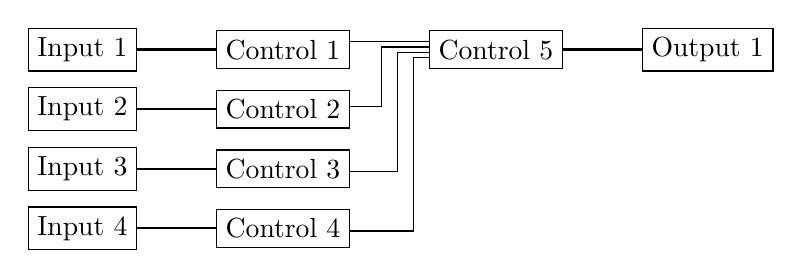
\begin{tikzpicture}
\node[rectangle,draw] (input1) {Input 1};
\node[below=2mm of input1,rectangle,draw] (input2) {Input 2};
\node[below=2mm of input2,rectangle,draw] (input3) {Input 3};
\node[below=2mm of input3,rectangle,draw] (input4) {Input 4};
\node[right=1cm of input1,rectangle,draw] (control1) {Control 1};
\node[right=1cm of input2,rectangle,draw] (control2) {Control 2};
\node[right=1cm of input3,rectangle,draw] (control3) {Control 3};
\node[right=1cm of input4,rectangle,draw] (control4) {Control 4};
\draw[thick] (input1) -- (control1);
\draw[thick] (input2) -- (control2);
\draw[thick] (input3) -- (control3);
\draw[thick] (input4) -- (control4);
\node[right=1cm of control1,rectangle,draw] (control5) {Control 5};
%\node[right=1cm of control2,rectangle,draw] (control6) {Control 6};
\draw ([yshift=1mm]control1.east) -- ++(0.2,0) |-([yshift=1mm]control5.west);
\draw ([yshift=0.33mm]control2.east) -- ++(0.4,0) |-([yshift=0.33mm]control5.west);
\draw ([yshift=-0.33mm]control3.east) -- ++(0.6,0) |-([yshift=-0.33mm]control5.west);
\draw ([yshift=-0.33mm]control4.east) -- ++(0.8,0) |-([yshift=-1mm]control5.west);
\node[right=1cm of control5,rectangle,draw] (output1) {Output 1};
%\node[right=1cm of control6,rectangle,draw] (output2) {Output 2};
\draw[thick] (control5) -- (output1);
%\draw[thick] (control6) -- (output2);
\end{tikzpicture}
\caption{Logic diagram of audio mixer}
\end{figure}

\begin{enumerate}
  \item Takes power from USB or 12V input jack (either one is fine, USB would be nice).
  \item Takes four stereo inputs, ideally as RCA jacks.
  \item Has volume controls for each of the inputs.
%  \item Has two separate volume outputs.
  \item Has a master volume control.
  \item Optionally, a second output channel (with an independent volume control).
%  \item Has independent master volume controls for each of the outputs.
  \item Based on the LF353 operational amplifier.
  \item Has to fit on a 10x10cm PCB at max for cheapest production costs.
\end{enumerate}

I came up with these specifications because this is what I need: I have multiple devices on my desk, including my desktop Mac Mini, my MacBook Pro, occasionally another laptop and my phone. Each of these devices should be able to send audio to my stereo system, but my stereo is very basic and has only one line-level input.

This device needs to be able to take audio from any of my devices, mix it together, and send it to either my stereo or my headphones. It does not need to do any amplification.

I chose the LF353 because it is available in a small but convenient form factor and relatively inexpensive. Also, SeeedStudio has it in stock.

\section{Research}

I did a bit of research while coming up with the specifications. I need to use some software to actually design the schematic and PCB. I also need to source parts, produce the PCB, and assemble the PCB.

\begin{enumerate}
  \item KiCAD (\url{http://www.kicad-pcb.org/}) is my tool of choice for PCB design.
  \item SnapEDA (\url{https://www.snapeda.com/}) has part outlines and models for KiCAD and is free to use.
  \item SeeedStudio (\url{https://www.seeedstudio.com/}) offers PCB manufacture, assembly, and parts that I might use.
  \item JLC PCB (\url{https://jlcpcb.com/}) offers afforcable PCB manufacturing.
  \item DigiKey has a large stock of electronic compounds.
  \item LCSC (\url{https://lcsc.com}) has a lot of low-cost components that can be shipped from china. Because it is based in asia, shipping takes a long time.
\end{enumerate}

It is important that I find good connectors and potentiometers that will last a while. For the case, I will find ideas after I have designed the PCB, since it is easy to 3D-print a case.

\section{Parts}

\subsection{RCA Connector}

I need five sets of two RCA connectors (one connect for each of the two stereo channel for every input and output, with four inputs and one output, that makes five). I browsed DigiKey for the most rubust and yet cost-effective option, and found a number of candidates.

The important criterions were  that it is stocked (such that I can order the parts and expect them within a reasonable time frame).

At first, I found a simple two-contact RCA input. With the discounted rate by ordering at least ten, this part would cost 5.40€ for all five channels. That is quite a bit more expensive that I had thought it would be.

\begin{center}
\begin{tabular}{@{}p{3cm}p{3cm}p{3cm}@{}}
%\toprule
\multirow{2}{3cm}{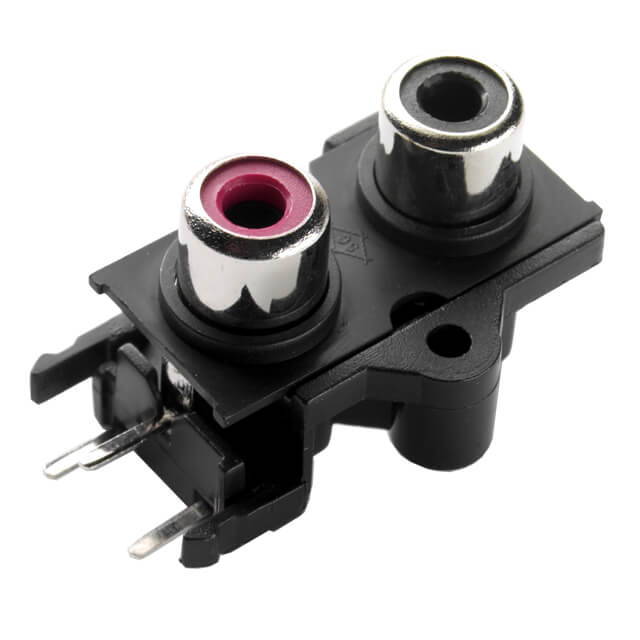
\includegraphics[width=3cm]{images/MFG_RCJ-22}}
& DigiKey Part & 102-5864-ND\\
& Manufacturer & CUI Devices\\
& Manufacturer Part & RCJ-2233\\
& Contacts & 2\\
& Price (1) & 1.23€\\
& Price (10) & 1.08€\\
%\bottomrule
\end{tabular}
\end{center}

Next, I was looking for bigger parts, thinking that it might potentially save money to buy larger. The one I found I thought looks really nice, with the metal and golden contacts. However, it does not seem to be cheaper than just using two simple 2-channel ones.

\begin{center}
\begin{tabular}{@{}p{3cm}p{3cm}p{3cm}@{}}
%\toprule
\multirow{2}{3cm}{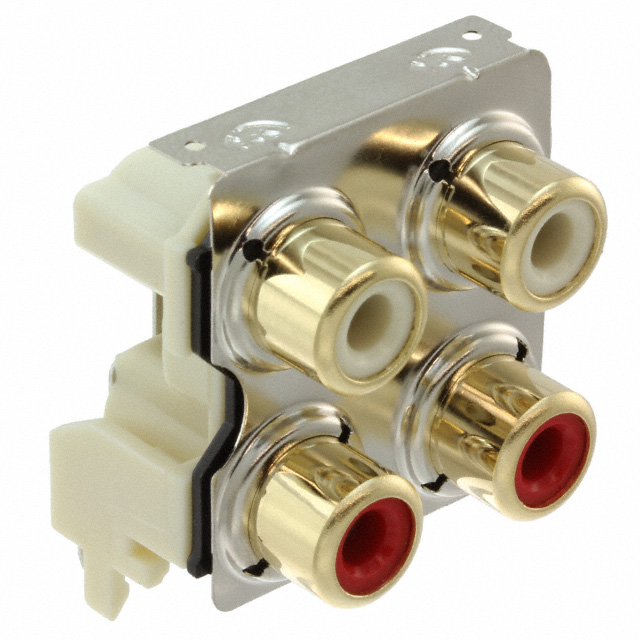
\includegraphics[width=3cm]{images/PJRAS2X2S01AUX}}
& DigiKey Part & SC2888-ND\\
& Manufacturer & Switchcraft Inc.\\
& Manufacturer Part & PJRAS2X2S01X\\
& Contacts & 4\\
& Price (1) & 2.88€\\
& Price (10) & 2.76€\\
%\bottomrule
\end{tabular}
\end{center}

When looking for even bigger ones, it seems like I found the one. An 8-input one that will do for all of the four stereo inputs, at only 3.79€.

\begin{center}
\begin{tabular}{@{}p{3cm}p{3cm}p{3cm}@{}}
%\toprule
\multirow{2}{3cm}{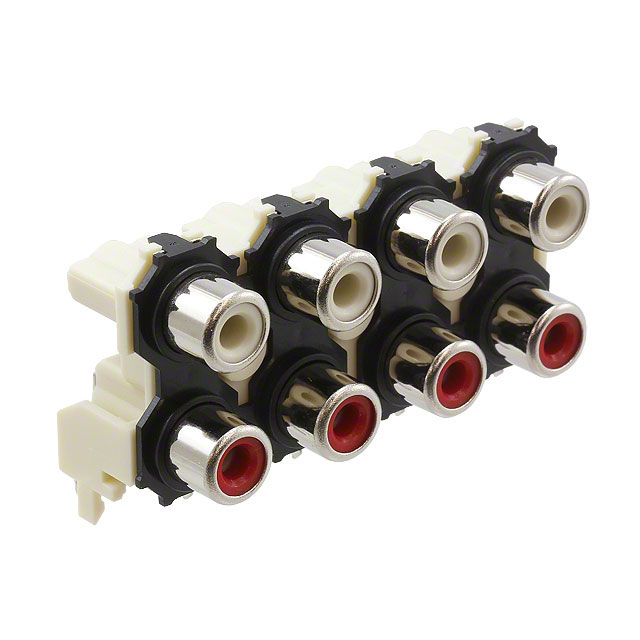
\includegraphics[width=3cm]{images/PJRAS4X2U01X}}
& DigiKey Part & SC1537-ND\\
& Manufacturer & Switchcraft Inc.\\
& Manufacturer Part & PJRAS4X2U01X\\
& Contacts & 8\\
& Price (1) & 3.79€\\
& Price (10) & 3.63€\\
%\bottomrule
\end{tabular}
\end{center}

\subsection{Opamps}

I need at least 10 opamps for the design that I have in mind -- one for every channel of the input (for 8 channels in total), plus one for every channel of the outputs (for an additional 2 channels).

The specifications state that I want to use the LF353 operational amplifier, however this is not a hard requirement. It is acceptable for me to use any other kind, as long as it is cheap, deliverable and works for audio applications. I exclude BGA parts from the search because I don't want to have too much issues in soldering them.

The prices I list here are the DigiKey prices, but I might end up sourcing them from SeeedStudio due to their assembly offer. 

\begin{center}
\begin{tabular}{@{}p{3cm}p{3cm}p{3cm}@{}}
%\toprule
\multirow{2}{3cm}{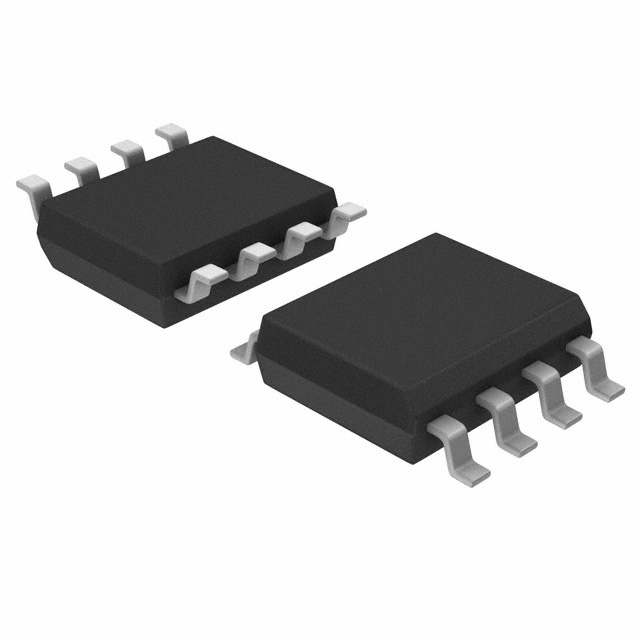
\includegraphics[width=3cm]{images/soic8}}
& DigiKey Part & 497-2967-1-ND\\
& Manufacturer & STMicroelectronics\\
& Manufacturer Part & LF353DT\\
& Opamps & 2\\
& Price (1) & 0.53€\\
& Price (10) & 0.44€\\
%\bottomrule
\end{tabular}
\end{center}

This first offer that I found is the one I was originally thinking about. It is offered by SeeedStudio and is, according to a single Google search, suitable for audio.

\begin{center}
\begin{tabular}{@{}p{3cm}p{3cm}p{3cm}@{}}
%\toprule
\multirow{2}{3cm}{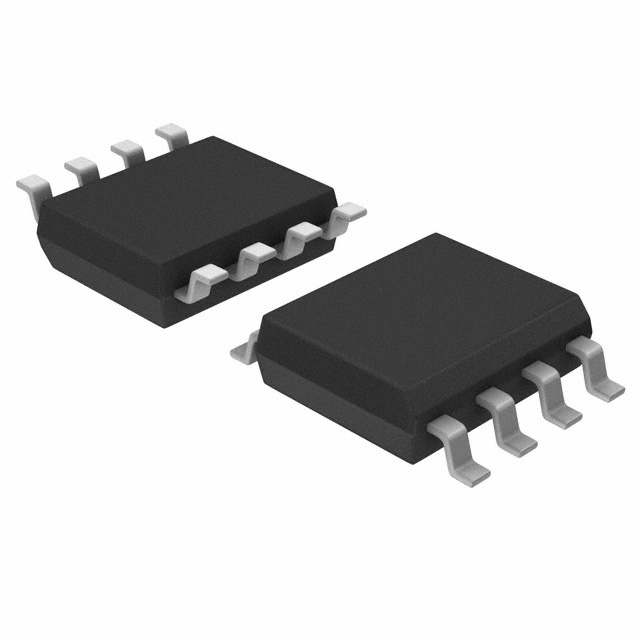
\includegraphics[width=3cm]{images/soic8}}
& DigiKey Part & 497-1597-1-ND\\
& Manufacturer & STMicroelectronics\\
& Manufacturer Part & LM833DT\\
& Opamps & 2\\
& Price (1) & 0.37€\\
& Price (10) & 0.31€\\
%\bottomrule
\end{tabular}
\end{center}

The second Opamp I found was one that is marked as being an amplifier specifically for audio on Digikey. The specs seem rather similar, I don't know what to make of most of them apart from the basics. But this one is cheaper, so I might go with it instead.

\begin{center}
\begin{tabular}{@{}p{3cm}p{3cm}p{3cm}@{}}
%\toprule
\multirow{2}{3cm}{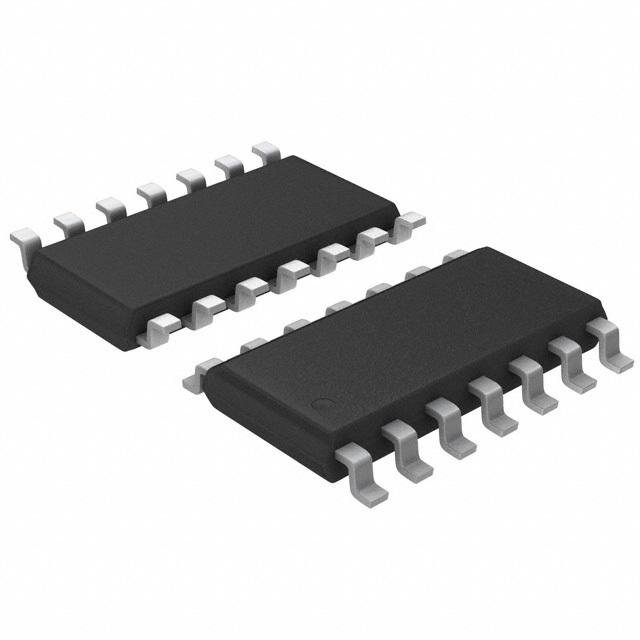
\includegraphics[width=3cm]{images/soic14}}
& DigiKey Part & 296-46621-1-ND\\
& Manufacturer & Texas Instruments\\
& Manufacturer Part & OPA1679IDR\\
& Opamps & 4\\
& Price (1) & 1.04€\\
& Price (10) & 0.88€\\
%\bottomrule
\end{tabular}
\end{center}

I also took a look at another operational amplifier with more channels. With the 2-channel opamps, I would need 5 ICs in total, which is maybe a bit much. Buying bigger packages means I can reduce the part count. This one is also suited to audio applications. However, it is more expensive than the LM833DT.

The main takeaway from the opamps is that I probably need a negative voltage rail. Ideally, I want something like a -12V and a +12V rail to give me a lot of headroom for the audio.

\begin{partdisplay}{soic8}
& Digikey Part & 296-13622-1-ND\\
& Manufacturer & Texas Instruments\\
& Manufacturer Part & NE5532DR\\
& Opamps & 4\\
& Price (1) & 0.77€\\
& Price (10) & 0.63€\\  
\end{partdisplay}

This last one I have added in the design phase as this was one that I was doing tests with. I happened to have some on hand, and it sounds very good. Although likely too expensive for the budget.

\subsection{Power Connector}

Choosing the right power connector is not an easy task. I have essentially two options.

\begin{itemize}
  \item Use a 12V barrel connector. This means I need an external power supply, which will cost additional money. However, this type of connector is ubiquitous, meaning that it will be easy to find parts. Also, power consumption like this is essentially unlimited.
  \item Use a USB connector. This might be more expensive. Also, power draw will be limited to 100mA unless I also use a chip to communicate to the other end that I need to draw more power. This will limit the voltage to 5V, meaning that I might need some logic to step up that voltage (and filter it to get a really clean supply).
\end{itemize}

I looked at both options to compare prices and see what is available. For the USB plug, I excluded USB type C due to the price as it is a newer standard.

\begin{partdisplay}{10118193-0001LF}
& DigiKey Part & 609-4616-1-ND\\
& Manufacturer & Amphenol ICC (FCI)\\
& Manufacturer Part & 10118193-0001LF\\
& Type & Micro USB\\
& Price (1) & 0.38€\\
& Price (10) & 0.36€\\
\end{partdisplay}

This first one I found I liked, it is inexpensive at 0.38€ and looks alright. I am a little worried about durability here, as these don't offer a clip to hold them down and provide extra strength.

\begin{partdisplay}{MFG_PJ-037A}
& DigiKey Part & CP-037A-ND\\
& Manufacturer & CUI Devices\\
& Manufacturer Part & PJ-037A\\
& Type & 2mm/5.5mm Barrel Jack\\
& Price (1) & 0.52€\\
& Price (10) & 0.48€\\
\end{partdisplay}

The second option I looked at is the ubiquitous barrel jack. This one is, as expected, a little bit more pricey. However, it does have the advantage of being able to deliver a lot of power easily.

\subsection{Power Supply}

Because line audio operates as AC with the neutral being grounded, and I need to build followers, I need a negative rail. There are different methods by which this can be achieved, the easiest way being a DC to DC converter. Since I don't need a lot of current, the easiest way here might also be the cheapest way.

\begin{partdisplay}{MFG_PDME1-S}
& DigiKey Part & 102-6321-ND\\
& Manufacturer & CUI Inc.\\
& Manufacturer Part & PDME1-S5-D9-S\\
& Input & 4.5-5.5V\\
& Output & 9V, -9V\\
& Power & 56mA\\
& Price (1) & 2.19€\\
& Price (10) & 2.15€\\
\end{partdisplay}

The first part I found looks very promising already. It takes in USB level voltage, and is able to deliver a ±9V power rail. It is only able to deliver 56mA, which should however be enough for the opamps. The only issue with it is the price — at 2.19€, it is a very expensive part. This part is also available in a ±12V version at the same price.

I also took a look at some ICs that I might be able to use to generate the supply rails, but found that it was not really practical, as I would need to use two additional ICs along with support circuitry. I might look into this another time.

\subsection{Potentionmeters}

The potentiometers that I use in this product need to be of high quality such as not to degrade or introduce unwanted audible artefacts. Also, I probably want to use logarithmic ones, to give the audio control a more linear feel. Last, I need the potentionmeters to be dual-channel. When first looking, I forgot about that.

\begin{partdisplay}{PDB182}
& Digikey Part & PDB182-K425K-103A-ND\\
& Manufacturer & Bourns\\
& Manufacturer Part & PDB182-K425K-103A\\
& Resistance & 10k ±20\%\\
& Type & Logarithmic\\
& Power & 0.06W\\
& Price (1) & 1.71€\\
& Price (10) & 1.50€\\
\end{partdisplay}

This one looks like those really cheap Chinese potentiometers, but I guess that is just how potentiometers look like. I'm surprised at how expensive it is -- this would add 8€ towards the cost of the product. I hope I can find a more economical alternative. While looking for other potentiometers, I learned that there are many kinds of precision potentiometers, some selling for three-figure amounts.

I also consider whether it might be better for me to use linear regulators, since I happen to have some that I have not yet put to good use. Another consideration is maybe using a digital potentiometer rather than a physical one, and implementing some kind of control via the serial port. That would change the scope of the project a bit, and to be honest, I do like the idea of having a physical knob to turn. 

\begin{partdisplay}{EVJY}
& Digikey Part & P2J4103-ND\\
& Manufacturer & Panasonic Electronical Components\\
& Manufacturer Part & EVJ-YK6F03651\\
& Resistance & 10k ±20\%\\
& Type & Logarithmic\\
& Power & 0.05W\\
& Price (1) & 1.93€\\
& Price (10) & 1.19€\\
\end{partdisplay}

The second one I found is even more expensive -- at least when buying a single one. However, the price is acceptable when buying more than 10 at a time. It also has a good form factor.

\begin{partdisplay}{soic6}
& Digikey Part & MCP4018T-103E/LTCT-ND\\
& Manufacturer & Microchip Technology\\
& Manufacturer Part & MCP4018T-103E/LT\\
& Resistance & 10k\\
& Type & Linear\\
& Positions & 128\\
& Interface & I\textsuperscript{2}C\\
& Price (1) & 0.34€\\  
\end{partdisplay}

Just to know what that is all about, I also took a look at some digital potentiometers. The first one that I found looks really good at first glance -- especially the price looks good. However, upon further thinking, I realised that it is linear. It is possible to fake a logarithmic scale with a linear digital potentiometer, but that means that it would be limited to 7 audio positions, which doesn't sound all that great.

\begin{partdisplay}{175-16-QSOP}
& Digikey Part & MAX5456EEE+-ND\\
& Manufacturer & Maxim Integrated\\
& Manufacturer Part & MAX5456EEE+\\
& Resistance & 10k\\
& Type & Logarithmic\\
& Positions & 32\\
& Potentiometers & 2\\
& Interface & UP/DOWN Pins\\
& Price (1) & 3.05€\\
& Price (10) & 2.74€\\
\end{partdisplay}

Lastly, I found a chip that would actually work as a digital potentiometer. It is quite expensive, far more than the physical potentiometers, at 3€ per stereo channel. It would undoubtedly be fun to play with this and a microcontroller -- but it is out of the price range at this point.

\subsection{Capacitors}

As this deals with audio things, I need to make sure to use plenty good capacitors, as any type of noise will be noticeable. The datasheets of the components I use prescribe what kind of filter capacitors I need.

\begin{partdisplay}{nichion47cap}
& Digikey Part & 493-1808-ND\\
& Manufacturer & Nichicon\\
& Manufacturer Part & UPW1E4R7MDD\\
& Type & Electrolytic\\
& Capacity & 4.7µF\\
& Price (1) & 0.21€\\
& Price (10) & 0.14€\\  
\end{partdisplay}

The first cap I found is the one I will use for the filter caps on the input stage of the DC to DC transformer. It's surprisingly expensive to buy caps on digikey, normally they should be a couple cents a pop at most. All of this stuff adds to the BOM cost, which is a bit concerning.

\begin{partdisplay}{samsung8050}
& Digikey Part & 1276-1066-1-ND\\
& Manufacturer & Samsung Electro-Mechanics\\
& Manufacturer Part & CL21B105KAFNNNE\\
& Type & Electrolytic\\
& Capacity & 1µF\\
& Price (1) & 0.10€\\
& Price (10) & 0.07€\\  
\end{partdisplay}

The next cap I found is a ceramic cap. This is for power smoothing on the output of the DC to DC converter.

\begin{partdisplay}{samsung8050}
& Digikey Part & 1276-1014-1-ND\\
& Manufacturer & Samsung Electro-Mechanics\\
& Manufacturer Part & CL21C101JBANNNC\\
& Type & Electrolytic\\
& Capacity & 100pF\\
& Price (1) & 0.09€\\
& Price (10) & 0.05€\\  
\end{partdisplay}

\subsection{Inductors}

Since the datasheet of the DC to DC converter calls for an inductor on the input side, I looked for inductors. 

\begin{partdisplay}{MFG_MLZ2012}
& Digikey Part & 445-6402-1-ND\\
& Manufacturer & TDK Corporation\\
& Manufacturer Part & MLZ2012M6R8WT000\\
& Inductance & 6.8µH\\
& Current & 350mA\\
& Sat. Current & 220mA\\
& Price (1) & 0.13€\\
& Price (10) & 0.11€\\
\end{partdisplay}

This inductor is the first one I found. It has an acceptable price, so I went with it.

\subsection{Resistors}

I will likely also need a bunch of resistors -- however, I am not listing these here, as they are cheap enough that I don't need to worry about sourcing them.

\section{Design}

Next, I start my actual design process. I have downloaded and installed the most up-to-date version of KiCad on my system, which I will use to design this product. I have also made an account over at SnapEDA in order to access their free parts database. I start out with downloading all the parts I'm using or considering and import them into KiCad. I also downloaded and installed the Digikey library, but I was unable to find a lot of the parts I needed in it.

\subsection{USB Power Input}

The USB Power Input side was quite straightforward. I used the part for the USB connector. Since I don't actually do anything USB-related, I don't need to do anything with the data pins. All I do is tap off the V\textsubscript{in}, SHIELD and GND pins, and add a cap between the power rail and ground for filtering.

\begin{center}
  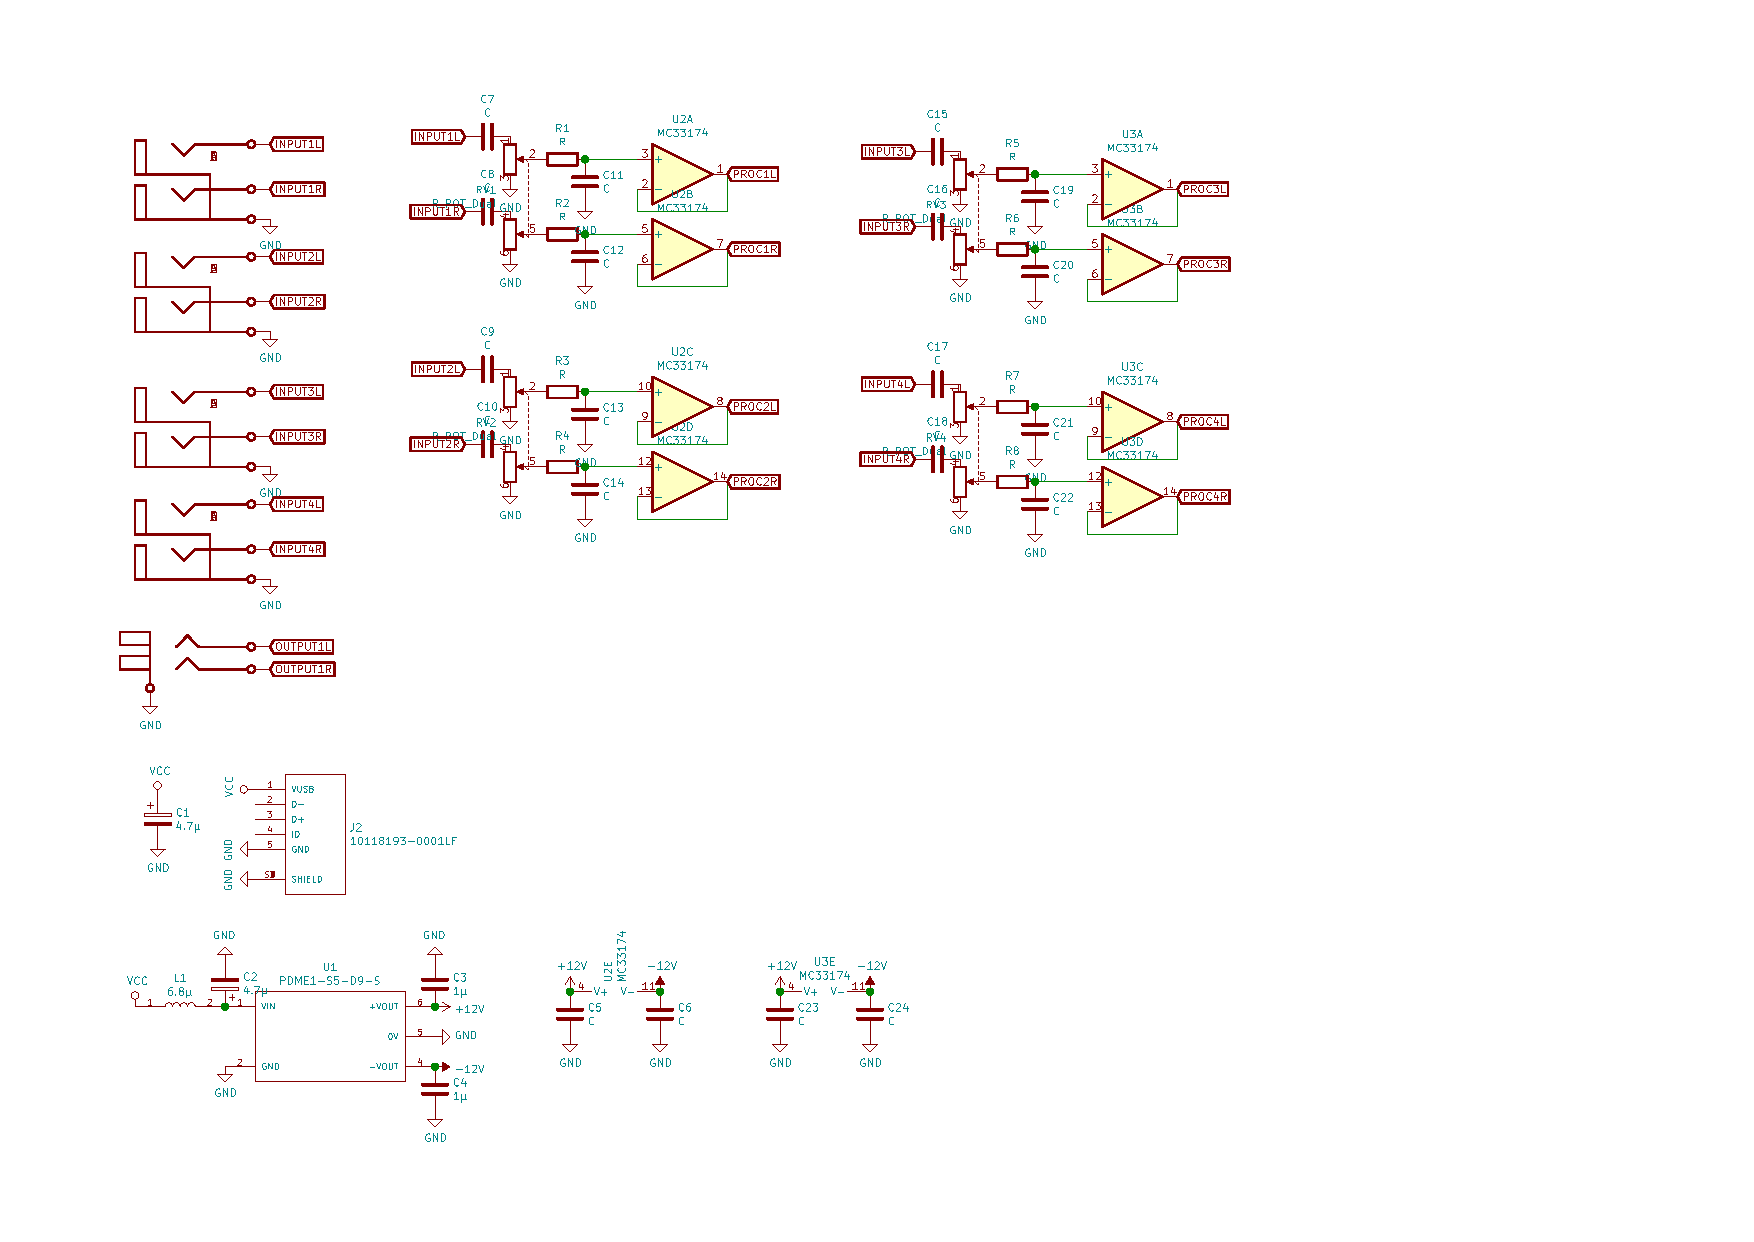
\includegraphics[trim={2cm 5.5cm 21cm 12.8cm},width=8cm,clip]{images/audio-mixer.pdf}
\end{center}

I might get back to this and add a fuse for protection, although I'm not sure yet if that is really necessary.

\subsection{Audio Jacks}

For the audio inputs (RCA Jacks), I simply added all eight (four stereo channels) of them. I attached their ground to the common ground, and created labels for every one of them.

\begin{center}
  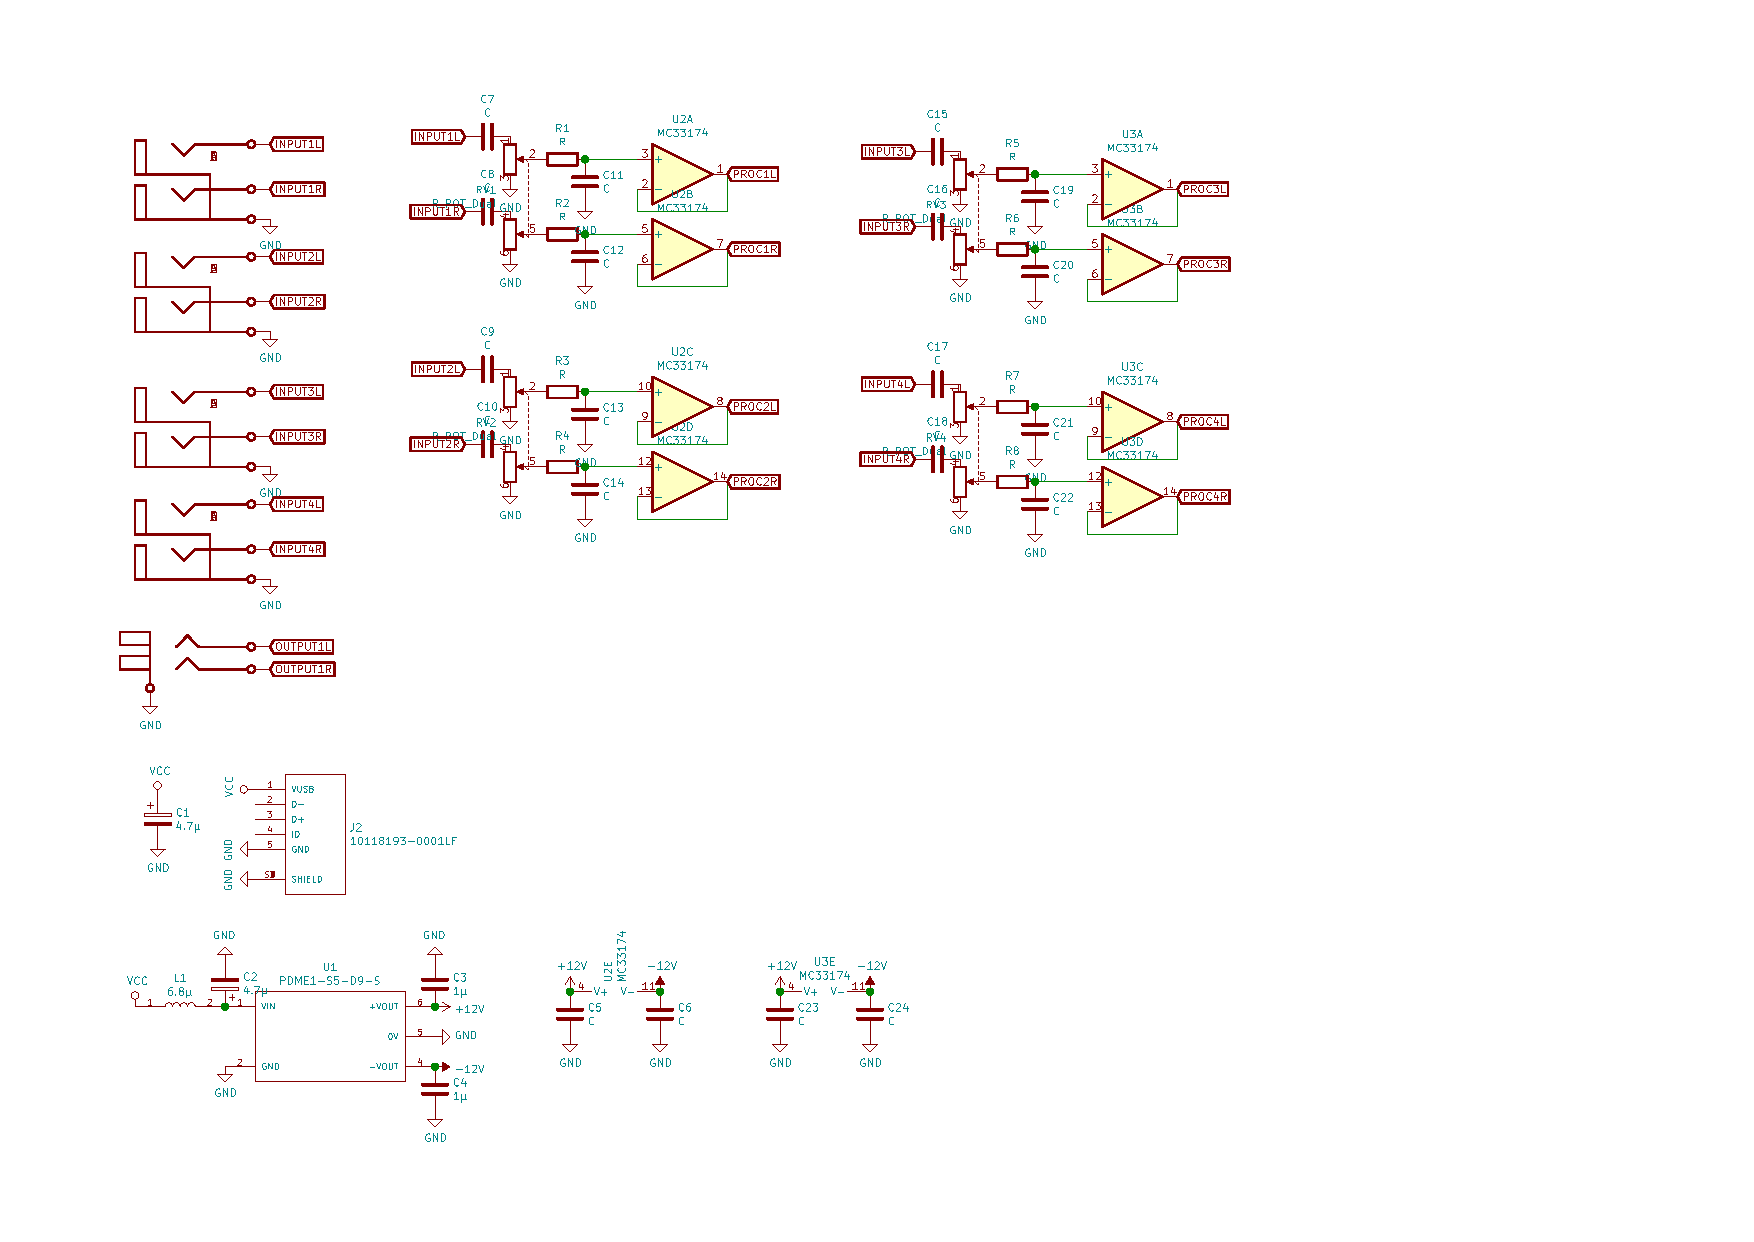
\includegraphics[trim={2cm 14.7cm 24cm 2cm},width=4cm,clip]{images/audio-mixer.pdf}
  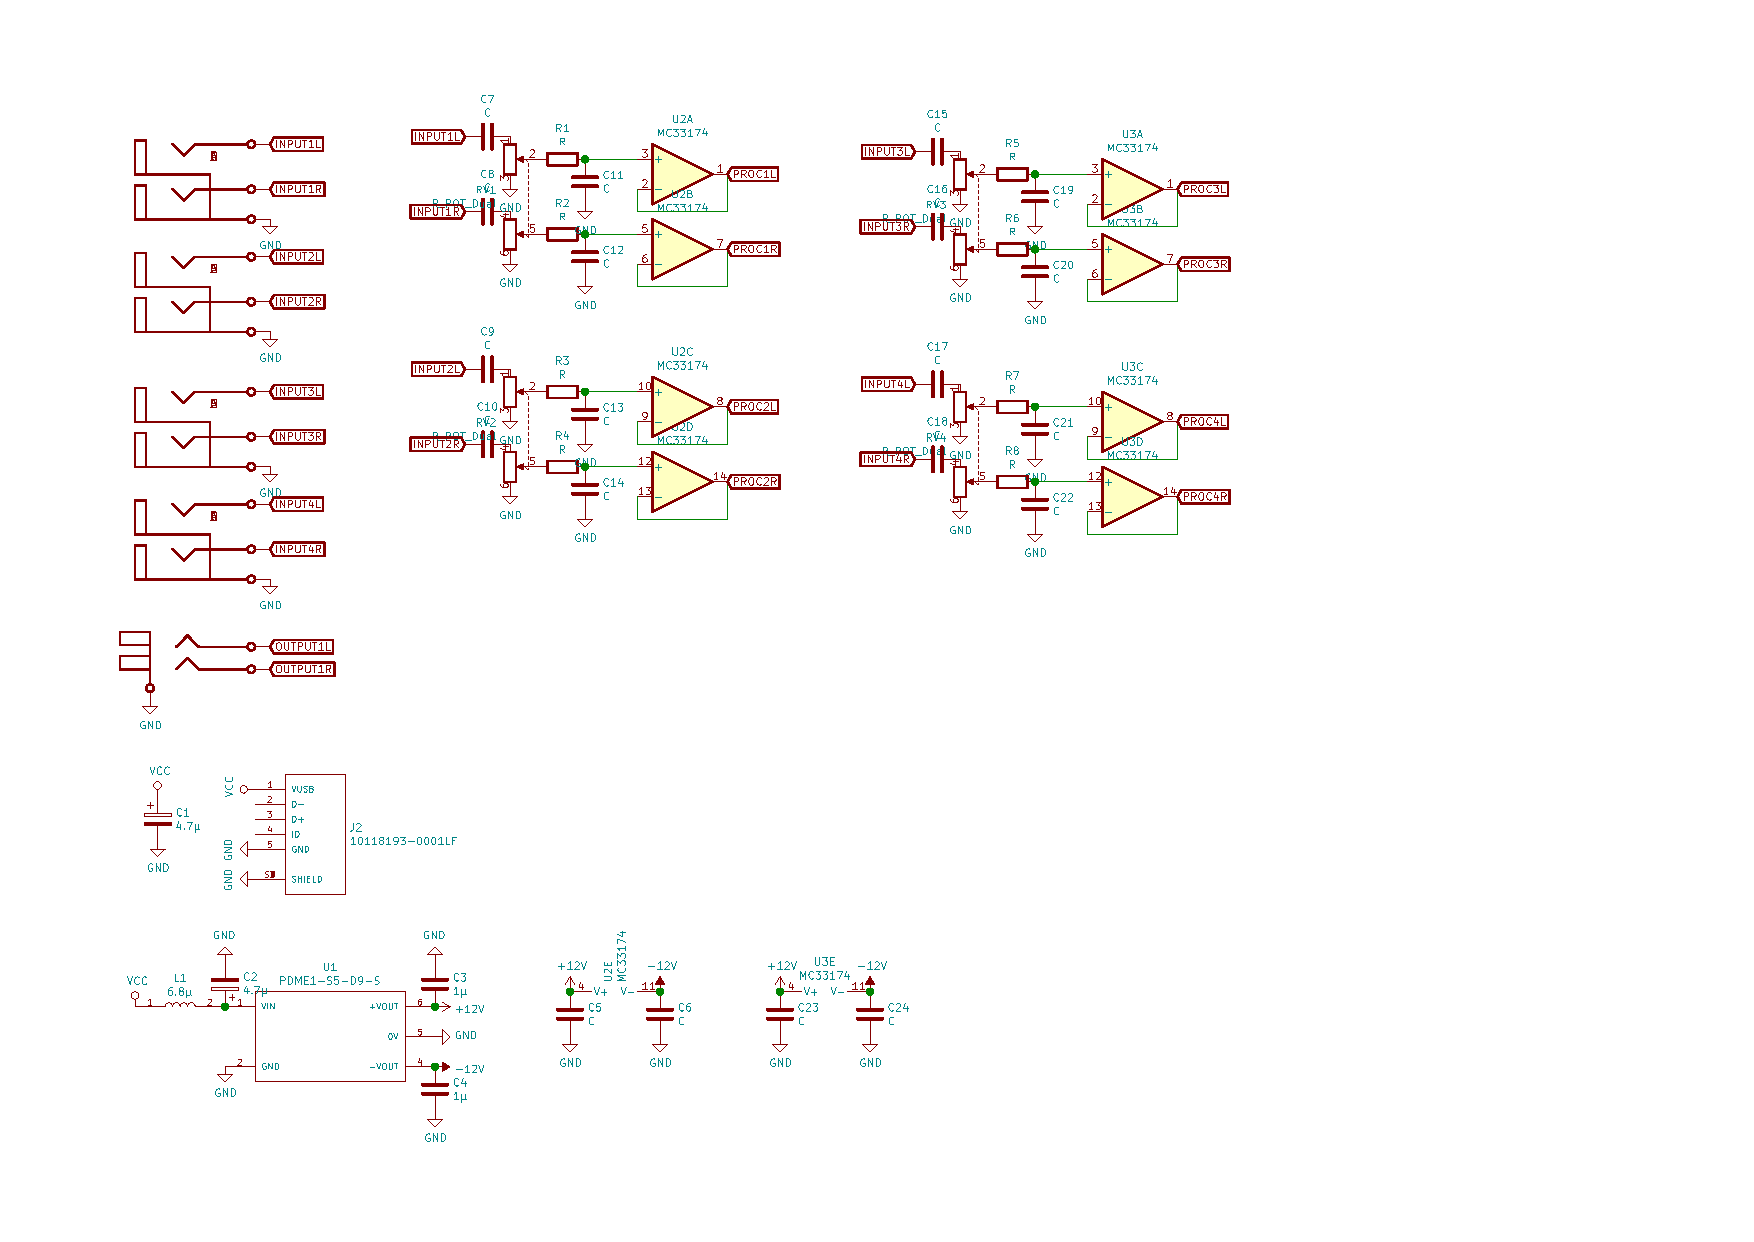
\includegraphics[trim={2cm 10.5cm 24cm 6.2cm},width=4cm,clip]{images/audio-mixer.pdf}
\end{center}

Likewise, I created an instance of the output jack in the schematic and set it up with the proper ground and labels.

\begin{center}
  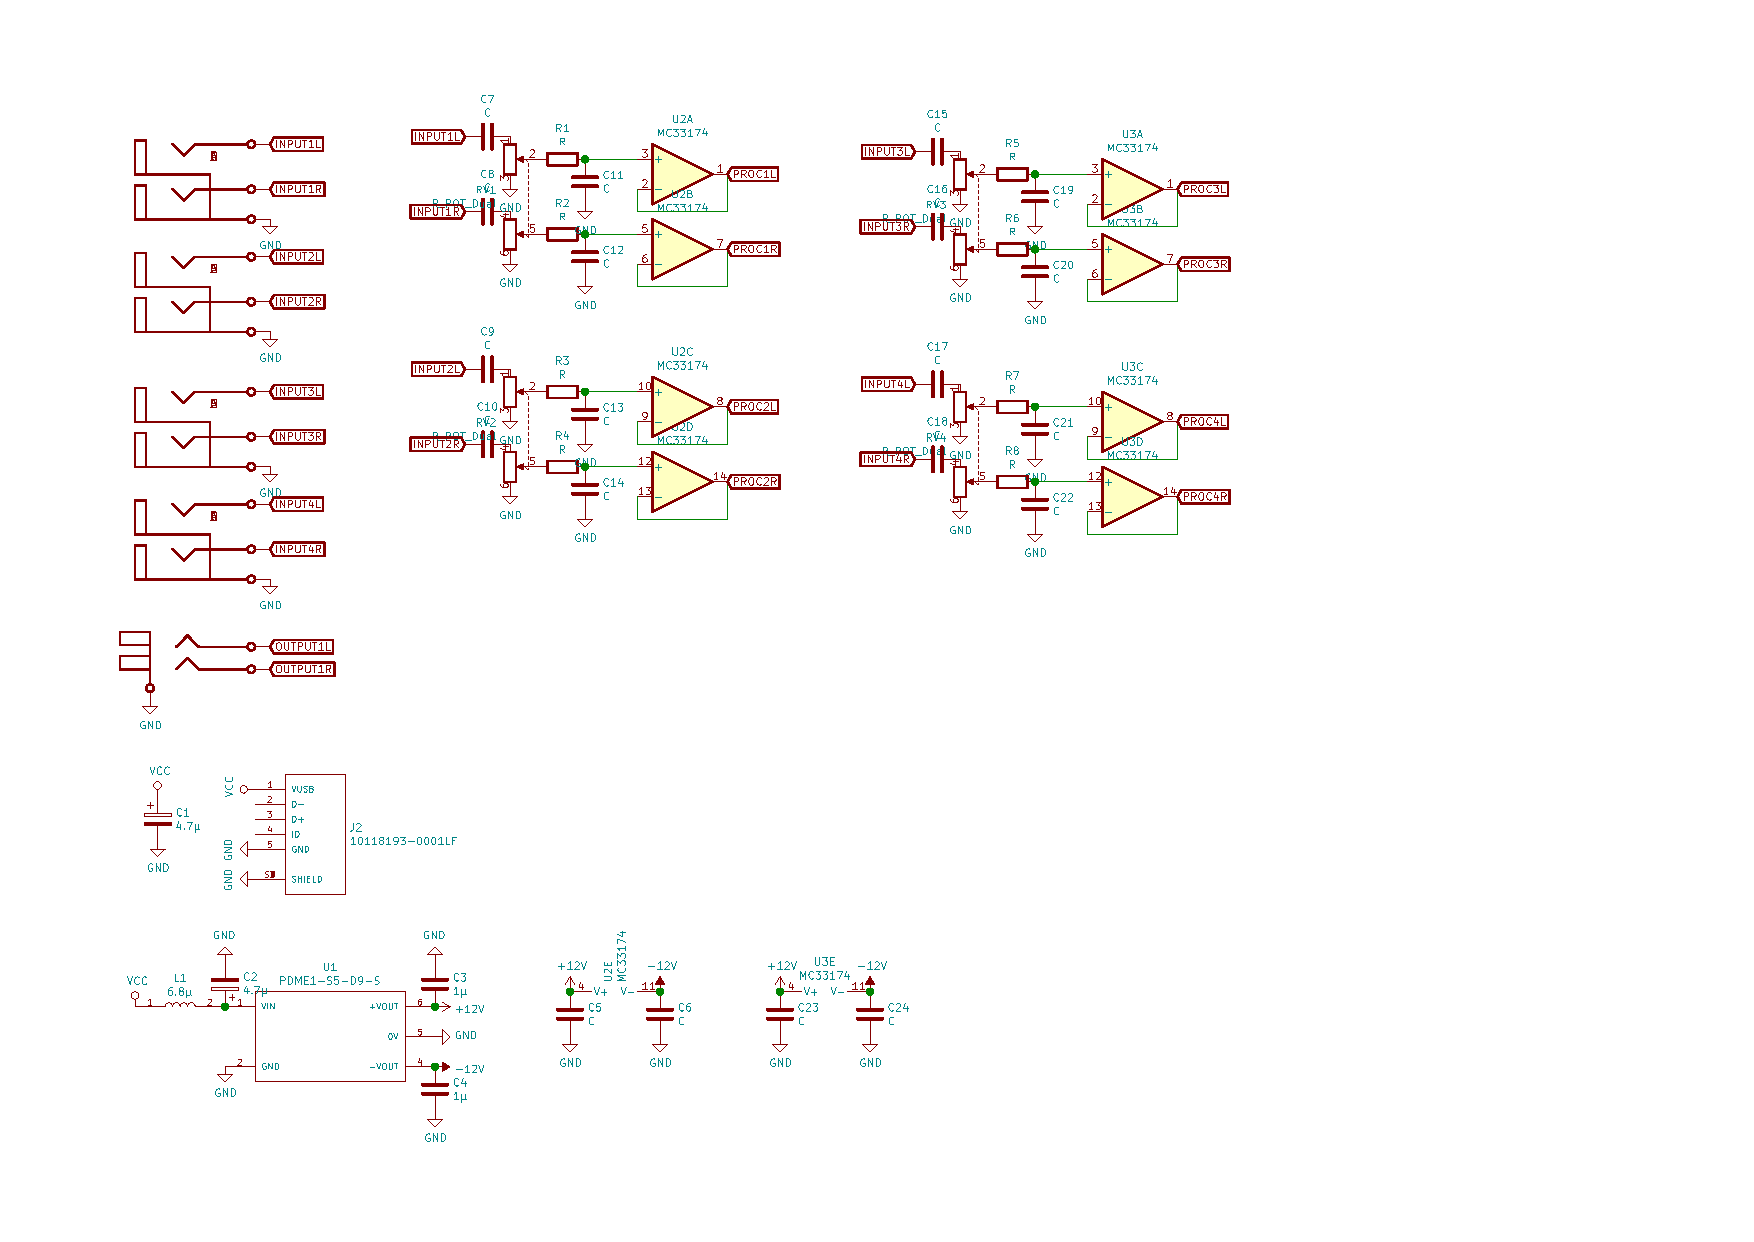
\includegraphics[trim={2cm 8.5cm 24cm 10.4cm},width=4cm,clip]{images/audio-mixer.pdf}
\end{center}

I have found the labels feature to be quite useful to prevent having to route excessive amounts of wires in the schematic, it helps keep things clean.

\subsection{DC to DC Power}

Next I designed the DC to DC Power stage. In this stage, I need to convert the \textasciitilde\SI{5}{\volt} from the USB into a ±\SI{9}{\volt} or ±\SI{12}{\volt} power rail used by the opamps. The reason I want a range like this is that the opamps will be used to make voltage followers, so they need to have a power rail that is in the range of the signal (which is ±\SI{2}{\volt} line level). It is always good to leave a bit of a margin just to be sure. Also, the opamps don't work too great too close to the rails.

\begin{figure}[h!]
\centering
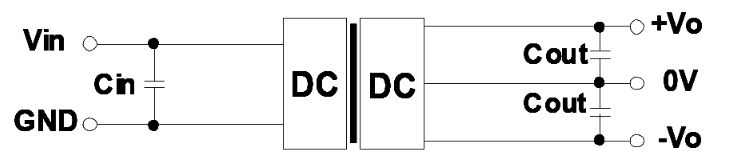
\includegraphics[width=6cm]{images/pdme-dual}
\caption{DC to DC converter dual rail setup}
\label{fig:pdme-dual}
\end{figure}

I first looked at the datasheet provided by the DC to DC converter, which has recommendation on how to use it in a circuit. Figure \ref{fig:pdme-dual} and \ref{fig:pdme-emc} show how the datasheet recommends setting it up, and this is what I followed.

\begin{figure}[h!]
\centering
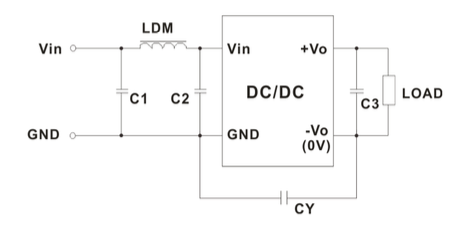
\includegraphics[width=7cm]{images/pdme-emc}
\caption{DC to DC converter EMC recommendation}
\label{fig:pdme-emc}
\end{figure}

The sample circuits are a little confusing, but I just implemented both of them as I thought it makes sense. I did omit $C_Y$ from Figure \ref{fig:pdme-emc} -- the device supports isolated outputs, but I chose to hook the output up to the ground, making the capacitor there redundant.

\begin{center}
  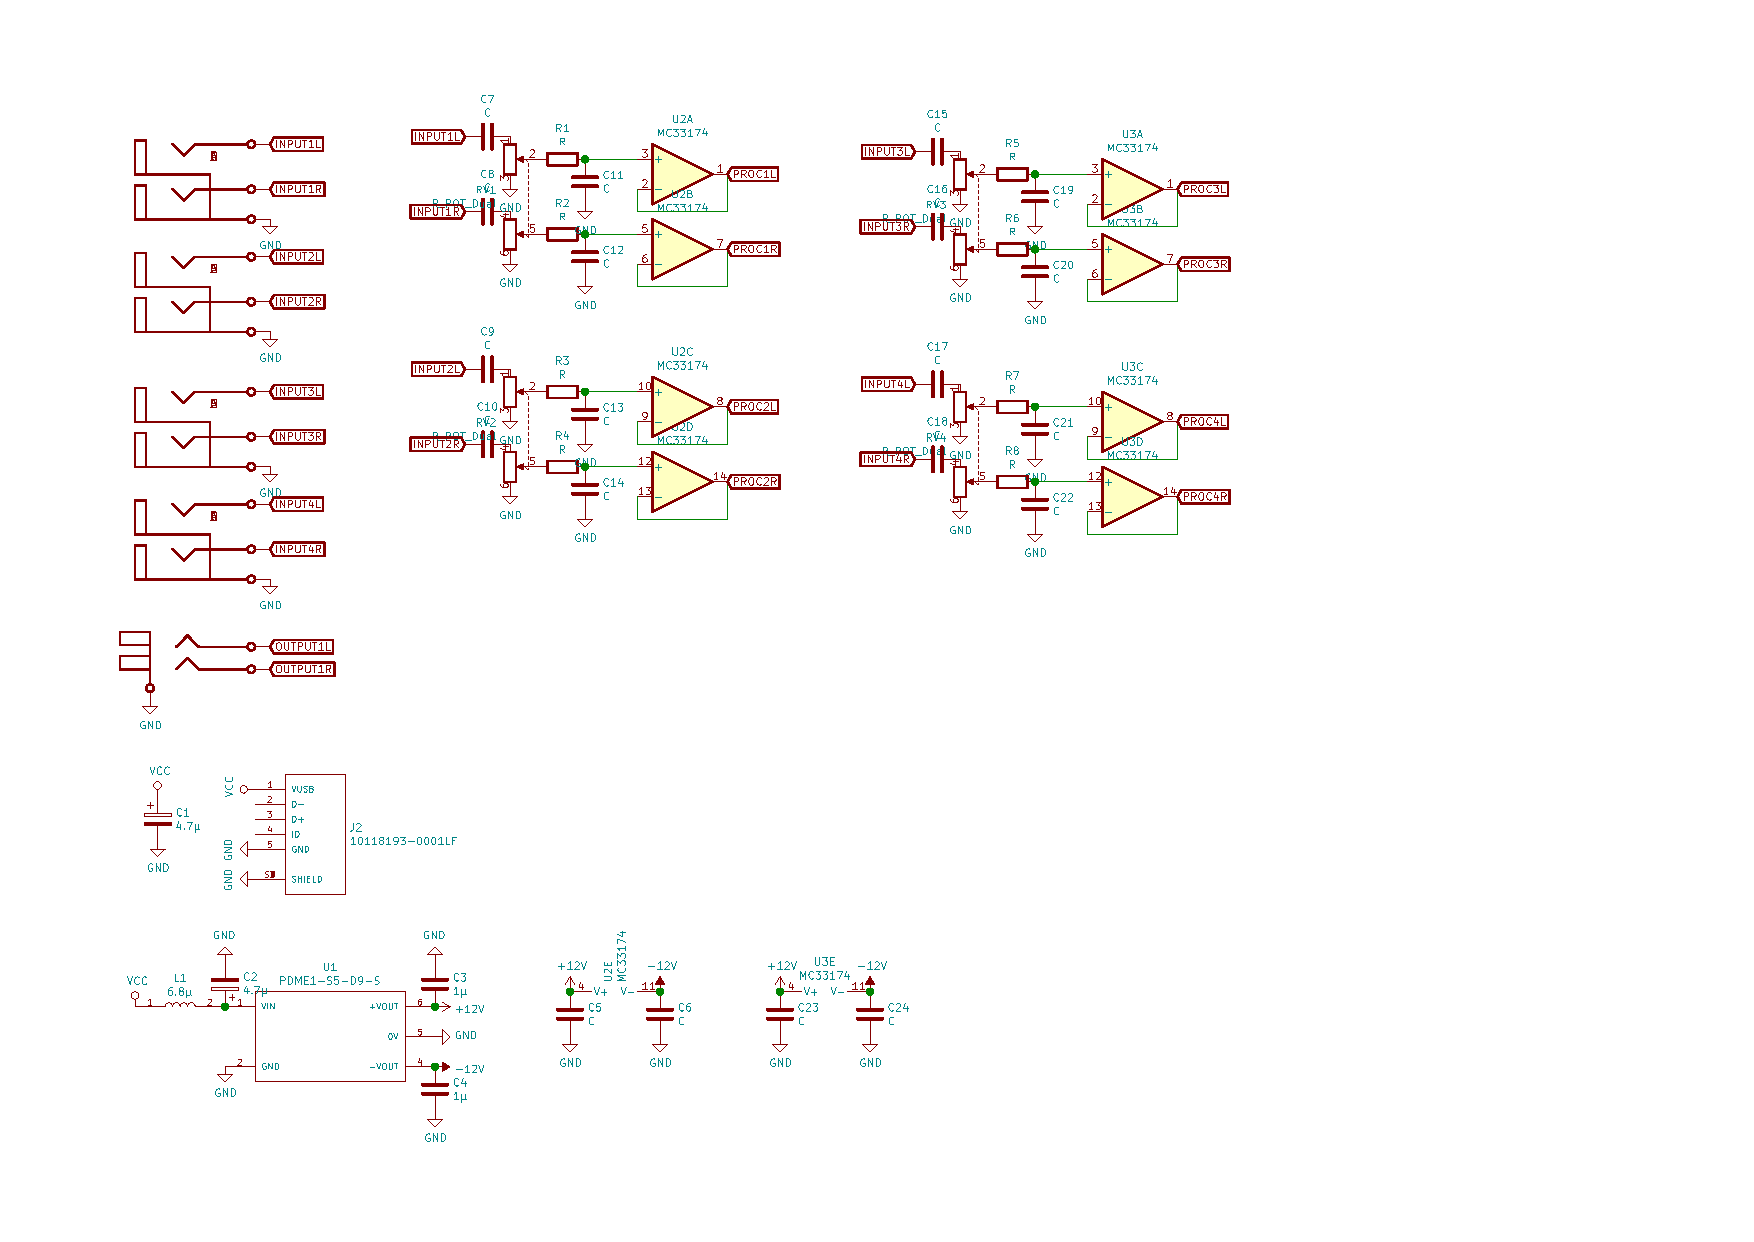
\includegraphics[trim={2cm 1.5cm 21cm 16cm},width=8cm,clip]{images/audio-mixer.pdf}
\end{center}

This is the result that I came up with. Note that the first capacitor, C1 in Figure \ref{fig:pdme-emc}, is not visible -- this can be seen on the USB Power Input side of things. I have labelled the two new power rails \verb|+12V| and \verb|-12V|, to differentiate from the existing V\textsubscript{cc} and GND rails.

\subsection{Audio Input Filtering}

For the actual money maker of this circuit, I had to do a bit more research. My idea is to use a setup something like this. For every individual mono channel on the input side.

\begin{center}
\begin{circuitikz}
\draw
  (0,0) node[anchor=east] {Input} 
    to ++(1,0) 
    to[potentiometer, name=pot] ++(0,-2)
    node[ground]{}
  (pot.wiper) to[highpass, name=hpf] ++(2,0) to ++(1,0)
    node[op amp, name=opamp,anchor=+]{}
  (opamp.-) -- ++(0,1) -- ++(2.4,0) to[short, -*] ++(0,-1.5)
  (opamp.out) -- ++(1,0) node[anchor=west] {Output}; 
\end{circuitikz}
\end{center}

With this, I would use the potentiometer directly at the input side of things to attenuate the signal, and then feed it though a highpass filter in order to remove any DC bias. The highpass filter should be setup to give me a \SI{-6}{\decibel} attenuation at \SI{10}{\hertz} (this is something I read online, and it makes sense to me). The opamp here is setup as a non-inverting follower. 

\subsubsection{Circuitlib Summing Amplifier}

While doing research, I stumbled upon a tutorial on circuitlib\footnote{\url{https://www.circuitlib.com/index.php/tutorials/product/39-how-to-build-an-audio-mixer}} that is built on the LM833 opamp, and has a similar setup to mine. 

\begin{center}
  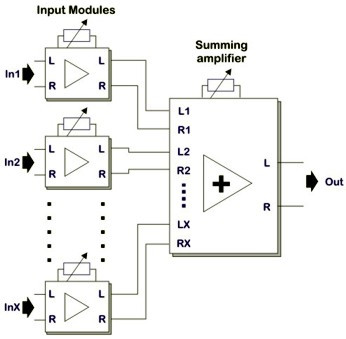
\includegraphics[width=5cm]{images/fig2_audio_mixer}  
\end{center}

The author uses a block-based setup, where the individual stereo channels are first processed and then all fed into a summing amplifier, much like I want to do.  This type of setup has the advantage that it is modular, meaning that it can easily be changed or extended, and it is testable, meaning that I can test the stages individually to make sure they sound good.

\begin{center}
  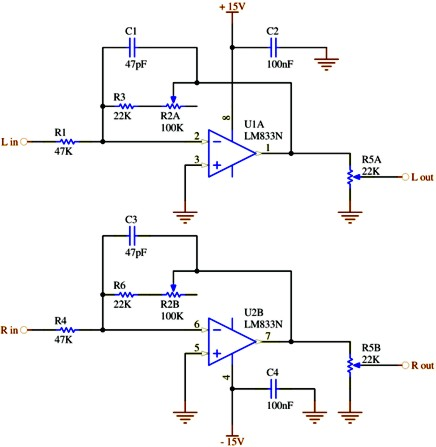
\includegraphics[width=7cm]{images/f3_audio_mixer}
\end{center}

The circuit the author uses for the input stage seems to make sense to me. It uses the opamps, and some circuitry to filter high-frequency noise above \SI{120}{\kilo\hertz}, this seems like it would be desireable. I don't yet see if this would also do DC rejection, but I will find out. So far, I like this design, it does not seem overly complicated.

\subsubsection{All About Circuits Summing Amplifier}

I also found an example circuit on All About Circuits\footnote{\url{https://www.allaboutcircuits.com/projects/build-an-audio-mixer/}}. This one is also rather similar to mine.

\begin{center}
  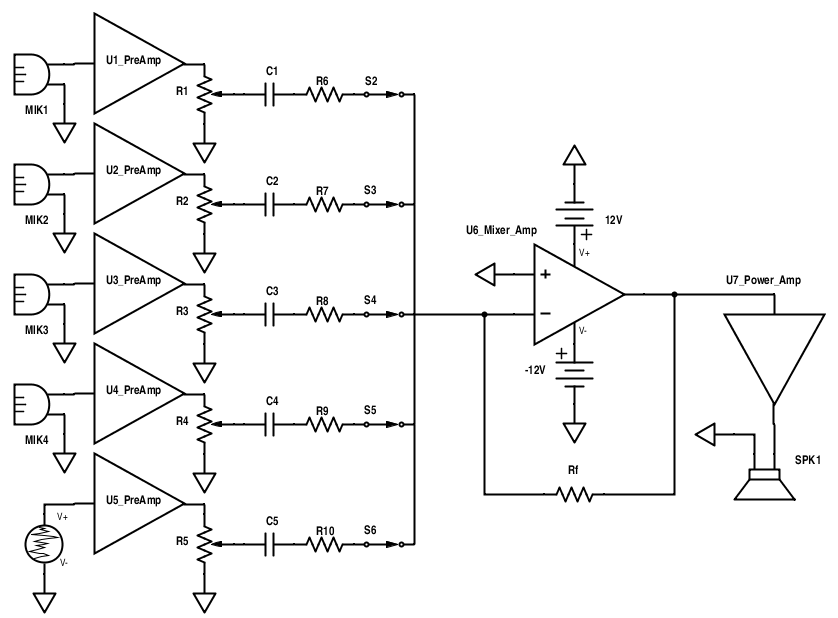
\includegraphics[width=8cm]{images/Audio-Mixer_8-5-2015}
\end{center}

What I like about this design is that it seems very simple, and what I like especially is that the author demonstrates some kind of simulation. I definitely would like to simulate and try out any potential designs before I build them. I am not sure what kind of software he uses for that simulation, but I will find out. 

What I dislike about this design is that he has not actually produced it, as far as I can tell, meaning that it is not clear if this works well in the real world.

\subsubsection{Experiments with LM358 and NE5532}

I created a simple experimental test setup, whereby I took music output from my iPhone, and fed it into a little circuit using an opamp. It included a simple potentiometer for voltage attenuation and an opamp set up as a unity gain amplifier (voltage follower). 

\begin{center}
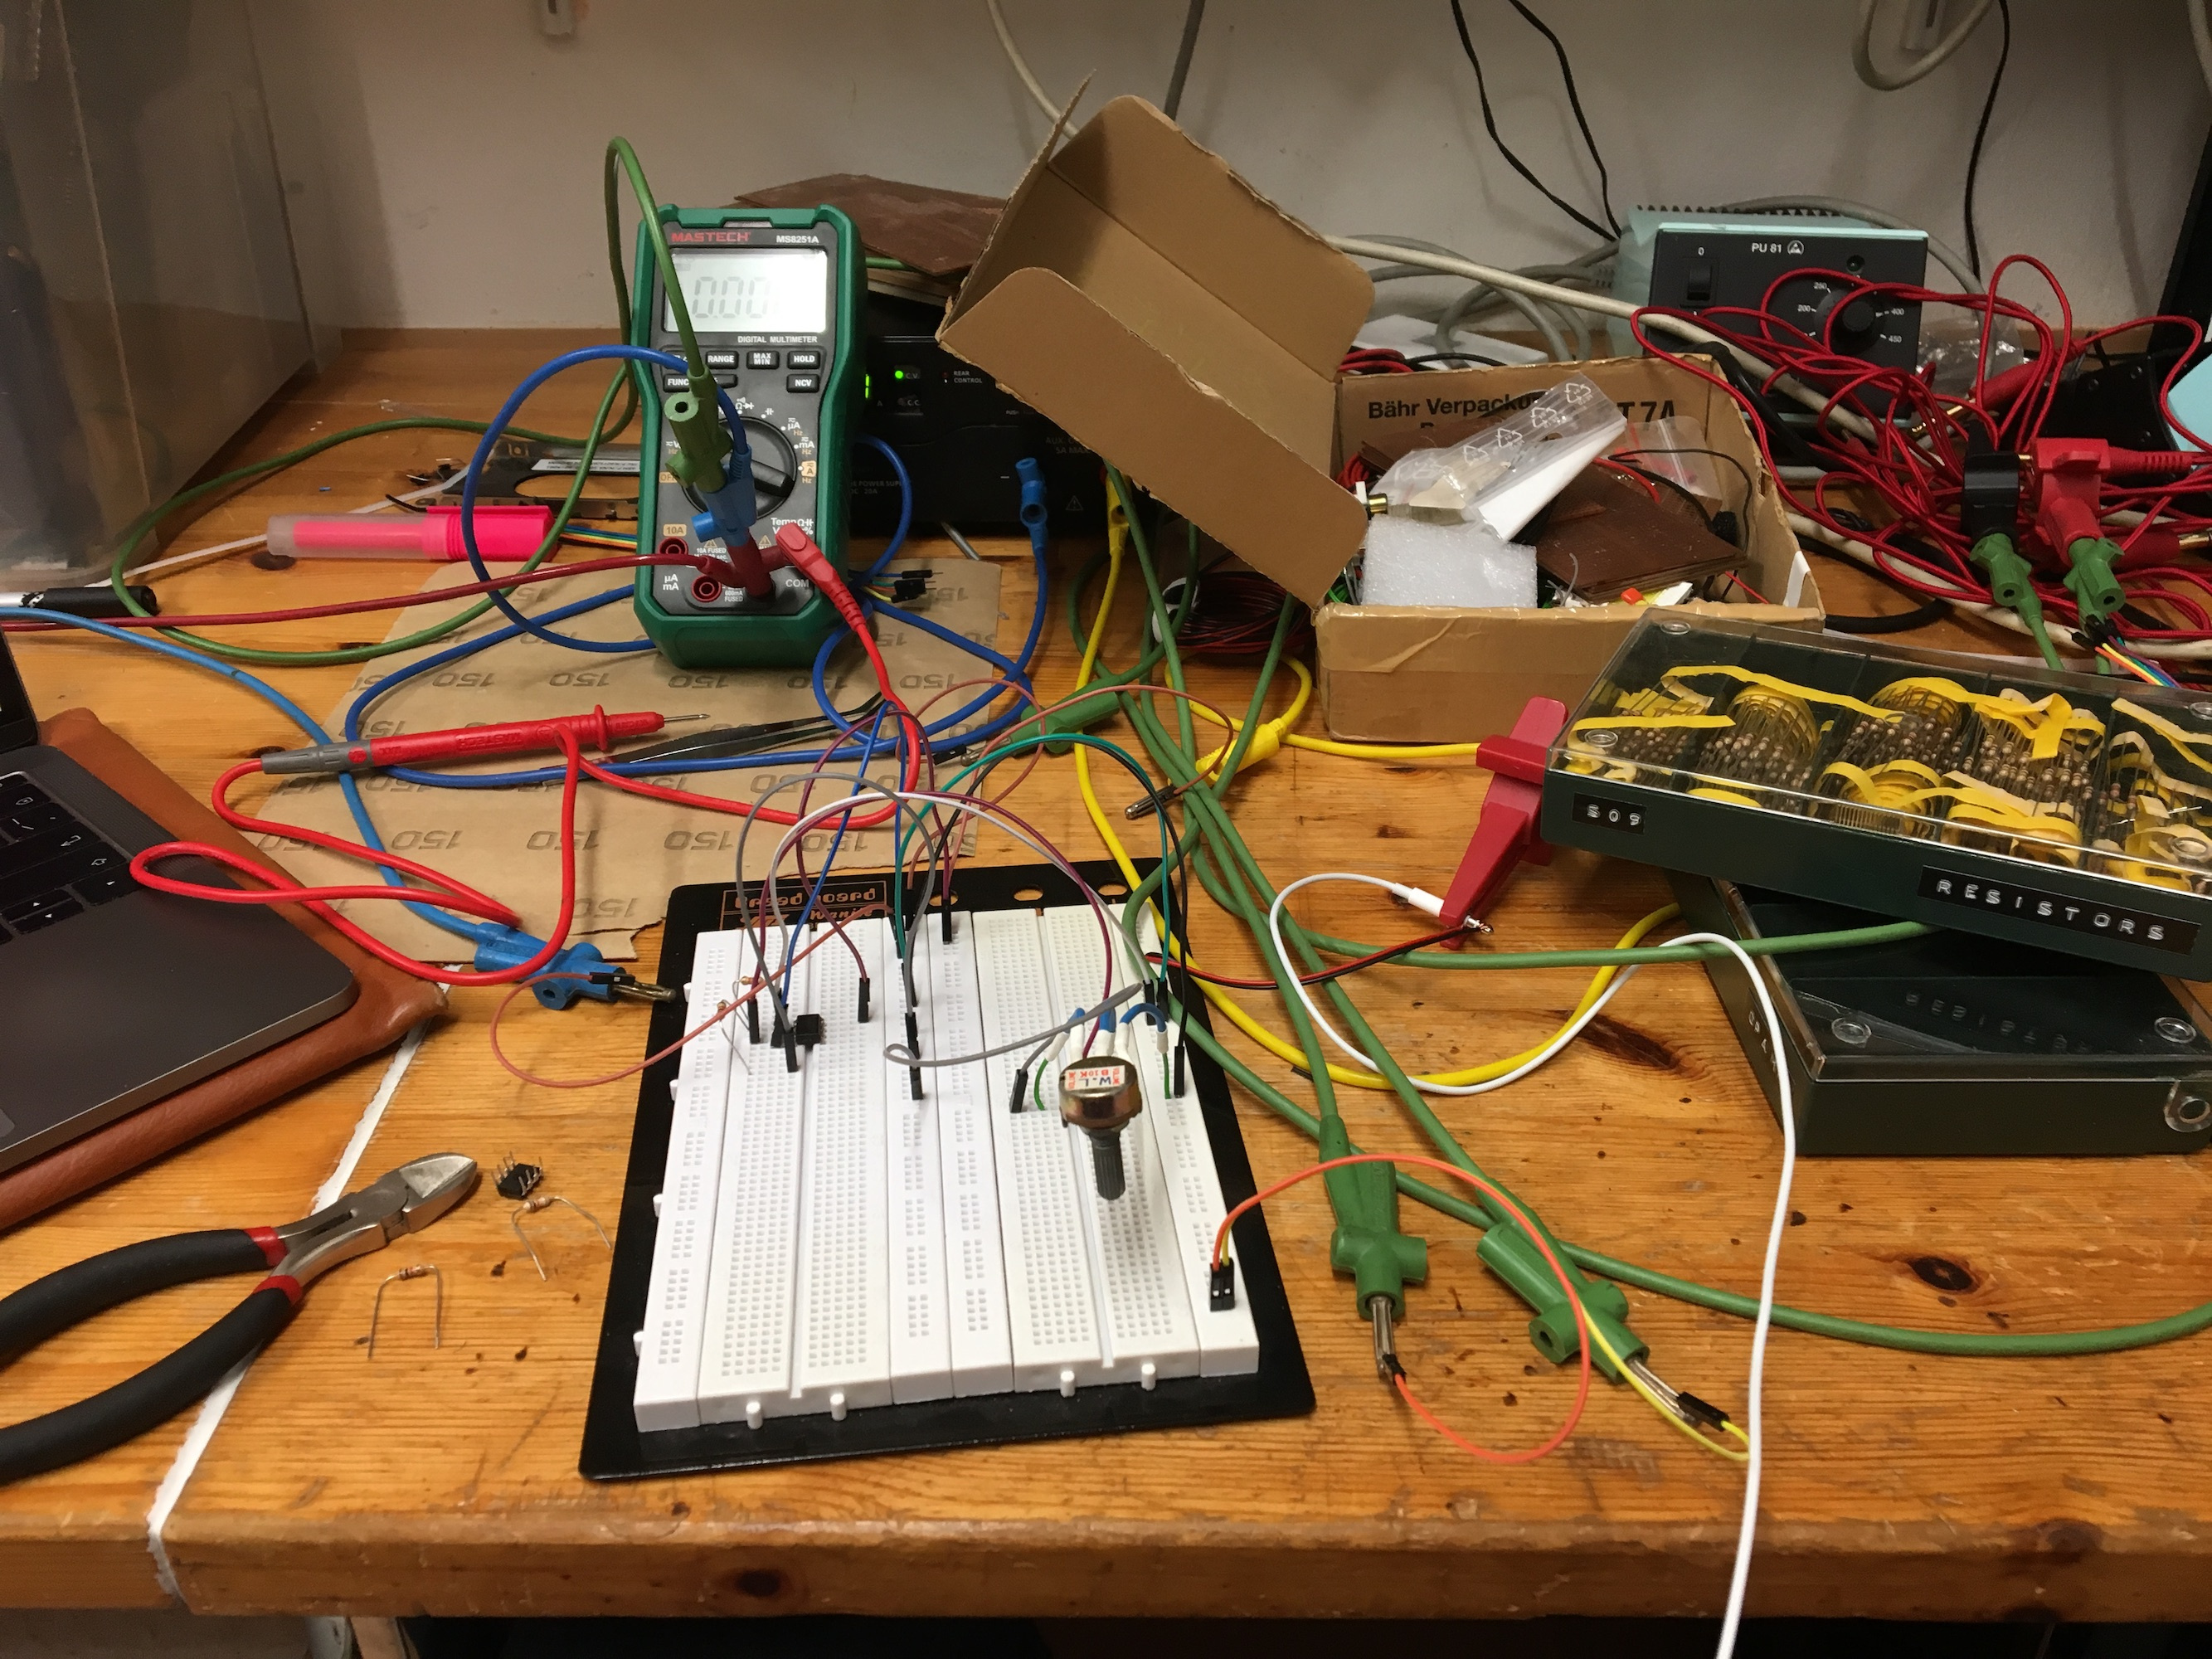
\includegraphics[width=7cm]{images/IMG_7757}  
\end{center}


I noticed a few things. First, there is noticeable hum when the opamp input is not connect to anything. This is mitigated by the potentiometer which will clamp it down to ground without an input. This is however also an issue with a long cable connected, which picks up interference. I don't know if there is some kind of circuit that might help here.

The other thing I noticed is that there is a (dramatic) difference in the sound produced by these two opamps! Without changing anything in the circuit, the NE5532 sounds good -- very crisp and clear. The LM358 however sounds very miserable. There must be some characteristic that it is lacking.

So far, I am satisfied with this simple experiment. It works better than I had expected. I am actually thinking of changing the circuit a bit now. If I reduce the impedance to something like \SI{1}{\kilo\ohm}, would that maybe reduce the humming noice perceived?

Reducing the impedance down to \SI{680}{\ohm} noticeably reduces the hum. I am happy with that result, hum should not be present in the input anywhere. I also did some research to find out how much these NE5532 opamps actually cost -- unfortunately, they are priced rather prohibitively, so I will likely not be using them in the product. It is however good to know that there is a difference in performance between different kinds, and I will make sure to test the ones I am looking to use. I found some\footnote{\url{http://nwavguy.blogspot.com/2011/08/op-amp-measurements.html}} discussions\footnote{\url{https://www.stereo.net.au/forums/topic/69927-the-lm833/}} about different kinds of opamps.

I used a website to calculate a value for a high-pass filter. I want to do DC rejection, and that is best done with a high-pass filter. For this, I can put a capacitor in line, the size of this depending on the impedance of the input (the size of the resistor). Using the tool, I found that with a \SI{680}{\ohm} resistor, values of around \SI{20}{\micro\farad} or \SI{10}{\micro\farad} are good, these will reject anything below around 10 or \SI{20}{\hertz}.

Next, I also considered using a low-pass filter to filter out high frequencies beyond the audible range.

\begin{center}
\ctikzset{label/align = smart}
\begin{circuitikz}[scale=0.7,every node/.style={scale=0.7}]
\draw
  (0,0) node[anchor=east] {Input}
  to[short,-o] ++(0,0)
  to[C,l=$C_1$,a=3.3<\micro\farad>,name=c1] ++(3,0)
  to[short,-*,name=x1] ++(0,0)
  to[R,l_=$R_1$,a^=680<\ohm>,name=r1] ++(0,-3)
  node[ground]{}
  (x1) to[R,l=$R_2$,a=1<\kilo\ohm>,name=r2] ++(3,0)
  to[short,-*] ++(0,0)
  to[short,-*,name=x2] ++(0,0)
  to[C,l_=$C_2$,a^=64<\nano\farad>,name=c2] ++(0,-3)
  node[ground]{}
  (x2) to ++(3,0)
  to[potentiometer, name=r3] ++(0, -3)
  node[ground]{}
  (r3.south) node[anchor=east,align=right,text width=1cm]{$R_3$\\\SI{10}{\kilo\ohm}}
  (r3.wiper) to ++(1,0)
  node[name=i1,op amp=$I_1$,anchor=+,yscale=-1]{}
  (i1.center) node{$I_1$}
  (i1.-) to ++(0,-1)
  to[R,l=$R_1$,a=1<\kilo\ohm>] ++(2.4,0)
  to[short,-*] ++(0,1.5)
  to[short,-o] ++(1,0)
  node[anchor=west] {Output};
\end{circuitikz}
\end{center}

The only issue with this circuit is that I read online that a line input should have an impedance of about \SI{10}{\kilo\ohm}. With this setup that I have here, that is not really the case. I am not sure how big of an issue this is, since a line output should probably be able to drive that. Also, it reduces susceptibility to interference from the cables.

After having done this experiment, I now understand more of how the circuit from circuitlib works. With that knowledge, and fixing the issue with the input impedance, I came up with this circuit.

\begin{center}
\ctikzset{label/align = smart}
\begin{circuitikz}[scale=0.7,every node/.style={scale=0.7}]
\draw
  (0,0) node[anchor=east] {Input}
  to[short,-o] ++(0,0)
  to[C,l=$C_1$,a=1<\micro\farad>,name=c1] ++(3,0)
  to[potentiometer,name=r1] ++(0,-3)
  to ++(0,-0.5)
  node[ground]{}
  (r1.south) node[anchor=east,align=right,text width=1cm]{$R_1$\\\SI{10}{\kilo\ohm}}
  (r1.wiper)
  to[R,name=r2,l=$R_2$,a=100<\kilo\ohm>] ++(3,0)
  to[short,name=x1,-*] ++(0,0)
  to ++(0,-1)
  to[C,l_=$C_2$,a^=50<\pico\farad>] ++(0,-1)
  node[ground]{}
  (x1) to ++(2,0)
  node[name=i1,op amp=$I_1$,anchor=+,yscale=-1]{}
  (i1.center) node{$I_1$}
  (i1.-) to ++(0,-1)
  to ++(2.4,0)
  to[short,-*] ++(0,1.5)
  to[short,-o] ++(1,0)
  node[anchor=west] {Output};
\end{circuitikz}
\end{center}

This circuit is more minimal and offers DC rejection. According to calculation and simulation, it has a \SI{3}{\decibel} loss at around \SI{10}{\hertz}. It also has a low-pass filter with a cutoff at around \SI{30}{\kilo\hertz}. Both of these filters are adjusted with the values of $C_1$ and $C_2$. The cutoff frequency also depends on the position of the volume potentiometer, but it only varies negligible amount.

\subsubsection{Choosing Opamps}

Now that I have bit of a feel for what is required to make a circuit, I have to choose which opamps I want to use in my product. I have already established that some opamps are not very suitable, such as the LM358. I would also like to use quad opamps in order to reduce BOM count.

One positive thing is that opamps seem to have more or less standardised pinouts. This means that I can design my circuit without knowing which specific opamp I will use, and I am able to change to using another type because their footprints will be compatible.

\begin{center}
\includegraphics[height=3cm,page=2,trim={11.6cm 19.8cm 5cm 3.2cm},clip]{datasheets/MC33272A-D.PDF}
\includegraphics[height=3cm,page=3,trim={3cm 11.4cm 12.2cm 11.9cm},clip]{datasheets/tl064.pdf}
\includegraphics[height=3cm,page=4,trim={7cm 18cm 7cm 2.8cm},clip]{datasheets/opa1679.pdf}
\end{center}

Taking price and specifications into consideration, I think the MC33272 is probably the ideal candidate. The specifications are good. I have not tried it yet, however.

\subsubsection{Final Schematic}

This is the final schematic I came up with. Note that in the schematic, I have used the MC33174 opamp, but this is only because a good part for it was available in the library. 

\begin{center}
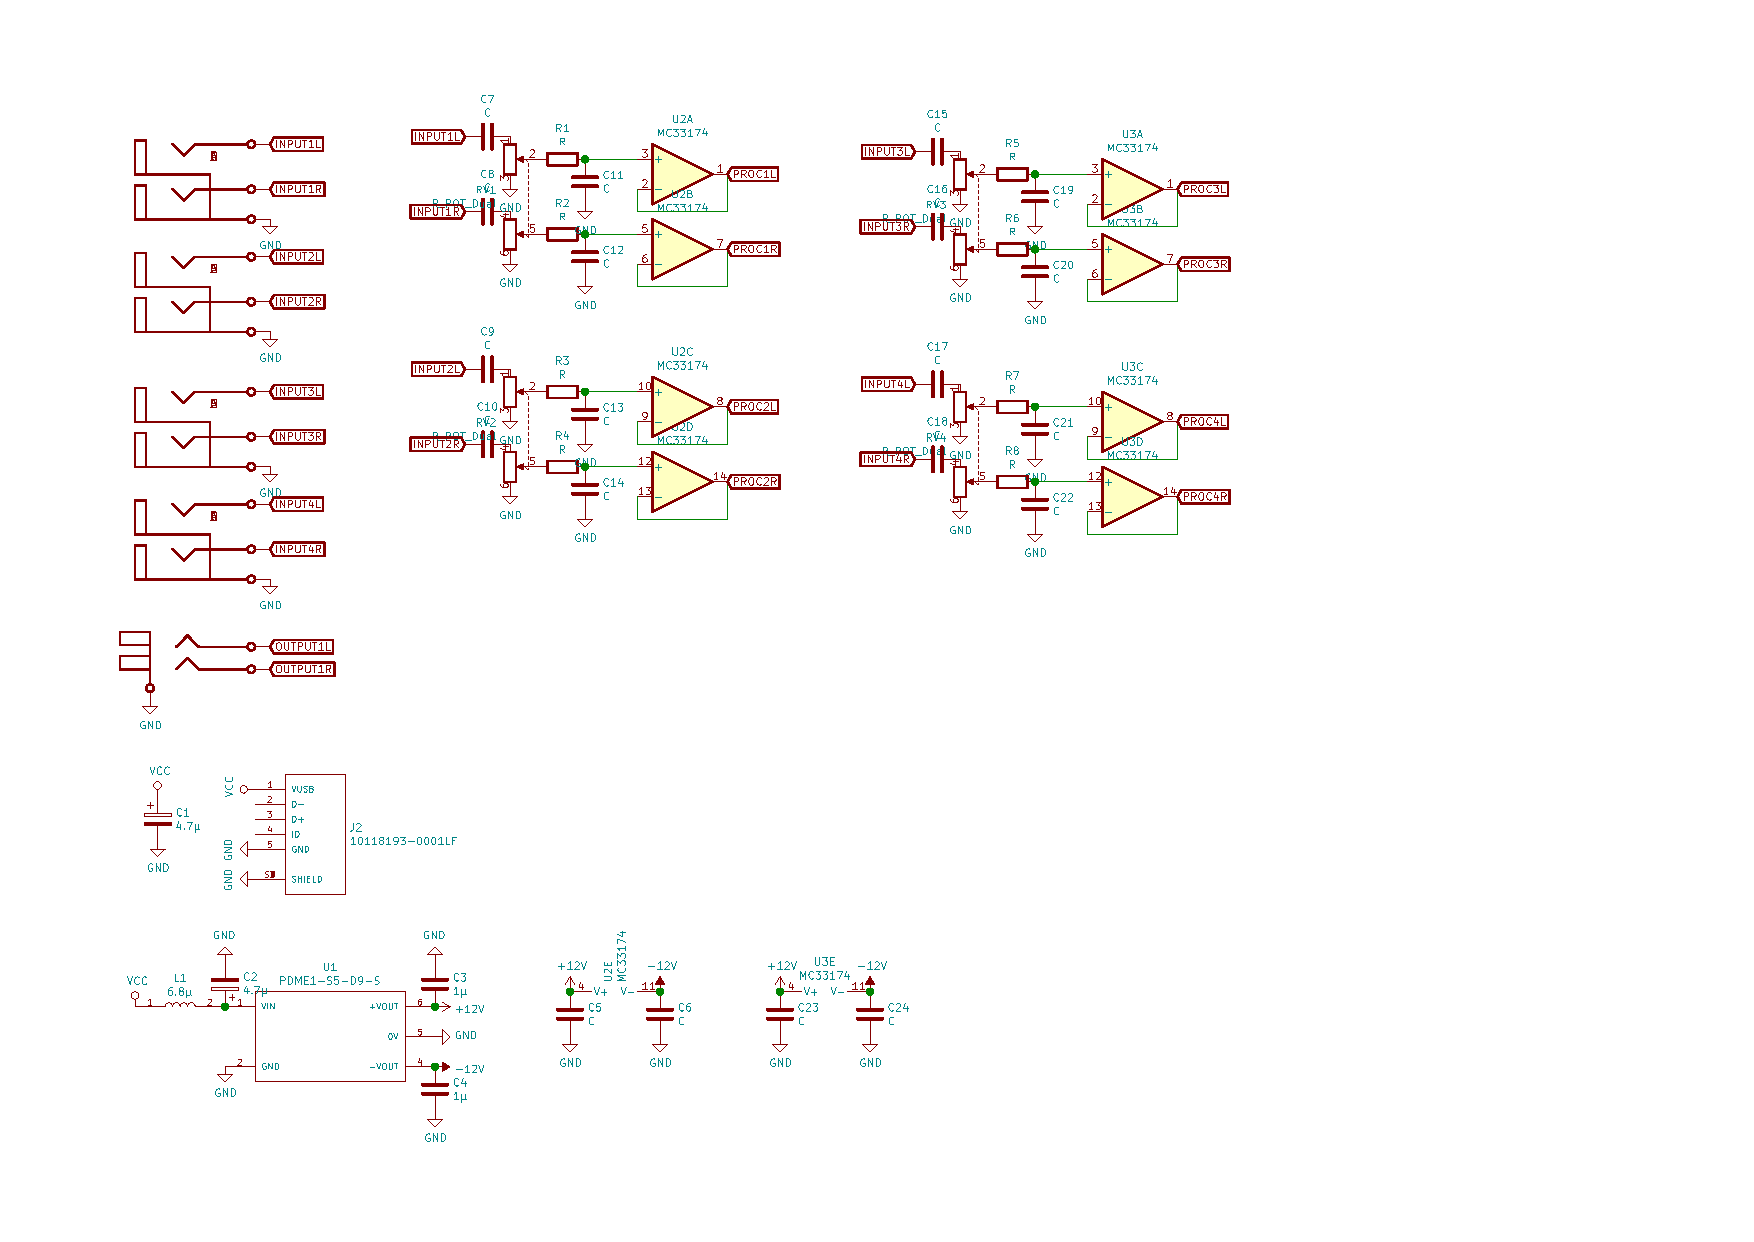
\includegraphics[trim={6.9cm 16cm 16.5cm 1.8cm},width=8cm,clip]{images/audio-mixer.pdf}
\end{center}

This is repeated for each of the four input channels. It looks a little crammed, I should leave a bit more space between the components. I like using labels to make circuits self-contained and to avoid having to route wires in the schematic. Here, the processed inputs get attached to a global label, \verb|PROC1L| and \verb|PROC1R|, which is then consumed by the mixing circuit. What is not visible in this part of the schematic is that I also have \SI{100}{\nano\farad} capacitors on the input rails of the opamps, going to ground.

\subsection{Audio Mixing}

Now that I figured out how to perform the audio input filtering, I have to actually mix the audio. The simplest way this can be achieved is with just a few simple resistors. The value of these needs to be chosen such that they provide proper impedance. My first idea was something like this.

\begin{center}
\begin{circuitikz}[scale=0.7,every node/.style={scale=0.7}]
\draw
  (0,0) node[anchor=east] {Input 1} 
    to[short,-o] ++(0,0)
    to ++(1,0) 
    to[resistor, name=R1, l=$R_1$] ++(1,0)
    to ++(1,0)
  (0,-1) node[anchor=east] {Input 2}
    to[short,-o] ++(0,0)
    to ++(1,0)
    to[resistor, name=R2, l=$R_2$] ++(1,0)
    to ++(1,0)
  (0,-2) node[anchor=east] {Input 3}
    to[short,-o] ++(0,0)
    to ++(1,0)
    to[resistor, name=R3, l=$R_3$] ++(1,0)
    to ++(1,0)
  (0,-3) node[anchor=east] {Input 4}
    to[short,-o] ++(0,0)
    to ++(1,0)
    to[resistor, name=R4, l=$R_4$] ++(1,0)
    to[short, -*] ++(1,0)
    to[short, -*] ++(0,1)
    to[short, -*] ++(0,1)
    to[short, -*] ++(0,1)
  (R1.right) to ++(2,0)
    to[potentiometer, name=pot, l_=$R_5$] ++(0,-2)
    node[ground] {}
  (pot.wiper) to ++(1,0)
    node[op amp, name=opamp,anchor=+,yscale=-1]{}
  (opamp.-) to ++(0,-1.5) 
    to[short,-*] ++(2.39,0)
  (opamp.out)
    to[R,l=$R_6$] ++(0,-2)
    to[R,l=$R_7$] ++(0,-2)
    node[ground]{}
  (opamp.out) to[short,-o] ++(1,0) node[anchor=west] {Output};
\end{circuitikz}
\end{center}

The idea here is that all inputs get summed up using resistors, and then I would use a potentiometer to attenuate the sum again, before sending it into the last opamp. This time, I don't want to set the op amp up with unity gain, I rather want it to compensate for the losses of the resistor divider. $R_6$ and $R_7$ should be set up such that a signal passed in on one of the inputs, with the other inputs connected to ground, should come out with the same level as it came in.

My original plan was to use $R_1 = R_2 = R_3 = R_4 = \SI{1}{\kilo\ohm}$ and $R_5 = \SI{10}{\kilo\ohm}$ for the potentiometer. However, calculations show that this causes an unacceptable power draw of \SI{6}{\milli\ampere} when two of the inputs are clamped to \SI{5}{\volt} and the other two to ground. This would be a peak current, but with a power budget of only \SI{40}{\milli\ampere}, it won't fly.

I have a few options here. I could use \SI{10}{\kilo\ohm} for the resistors, which would reduce the signal, meaning that I would have to compensate by increasing the amplification, or I could also change the potentiometer to a \SI{100}{\kilo\ohm} one. The issue with changing the pot is that it is a rather expensive part, and by having two different kinds, I can profit less from buying in bulk.

I decided to use $R_1 = R_2 = R_3 = R_4 = \SI{10}{\kilo\ohm}$ for the resistors, $R_5 = \SI{10}{\kilo\ohm}$ for the potentiometer, and $R_6 = \SI{10}{\kilo\ohm}$ and $R_7 = \SI{2.4}{\kilo\ohm}$ for the gain control resistor divider. With these values, losses from the resistors should be less than \SI{1}{\milli\ampere} with two inputs clamped to \SI{5}{\volt} and the others clamped to ground.

Since this circuit is simpler than I had anticipated, it would be possible to include it twice, for two separate outputs. This could potentially provide a headphone port. That would be possible without increasing the part count by adding a second potentiometer at the resistor adder, and changing the value of one of the gain control resistors.

\begin{center}
\begin{circuitikz}[scale=0.7,every node/.style={scale=0.7}]
\draw
  (0,0) node[anchor=east] {Input 1} 
    to[short,-o] ++(0,0)
    to ++(1,0) 
    to[resistor, name=R1, l=$R_1$] ++(1,0)
    to ++(1,0)
  (0,-1) node[anchor=east] {Input 2}
    to[short,-o] ++(0,0)
    to ++(1,0)
    to[resistor, name=R2, l=$R_2$] ++(1,0)
    to ++(1,0)
  (0,-2) node[anchor=east] {Input 3}
    to[short,-o] ++(0,0)
    to ++(1,0)
    to[resistor, name=R3, l=$R_3$] ++(1,0)
    to ++(1,0)
  (0,-3) node[anchor=east] {Input 4}
    to[short,-o] ++(0,0)
    to ++(1,0)
    to[resistor, name=R4, l=$R_4$] ++(1,0)
    to[short, -*] ++(1,0)
    to[short, -*] ++(0,1)
    to[short, -*] ++(0,1)
    to[short, -*] ++(0,1)
    to[short] ++(0,-3)
    to[short] ++(1.06,0)
    to[potentiometer, name=R8,l_=$R_8$] ++(0,-3)
    node[ground]{}
  (R1.right) to ++(2,0)
    to[potentiometer, name=R5, l_=$R_5$] ++(0,-2)
    node[ground] {}
  (R5.wiper) to ++(1,0)
    node[op amp, name=I1,anchor=+,yscale=-1]{}
  (I1.-) to ++(0,-1.5) 
    to[short,-*] ++(2.39,0)
  (I1.out)
    to[R,l=$R_6$] ++(0,-2)
    to[R,l=$R_7$] ++(2,0)
    node[ground]{}
  (I1.out) to[short,-o] ++(1,0) node[anchor=west] {Output 1}
  (R8.wiper) to ++(1,0)
    node[op amp, name=I2,anchor=+,yscale=-1]{}
  (I2.-) to ++(0,-1.5) 
    to[short,-*] ++(2.39,0)
  (I2.out)
    to[R,l=$R_9$] ++(0,-2)
    to[R,l=$R_{10}$] ++(2,0)
    node[ground]{}
  (I2.out) to[short,-o] ++(1,0) node[anchor=west] {Output 2};
\end{circuitikz}
\end{center}

With this setup, I have to let $R_6 = R_9 = \SI{10}{\kilo\ohm}$ and $R_7 = R_{10} = \SI{2}{\kilo\ohm}$ in order to compensate for the addition. I have decided to go with this for two reasons. It is more economical and practical to buy quad opamps, so if I use them exclusively (which would be optimal to reduce part count), I would have two spare anyways. It does add some cost for potentiometers and connectors, but I feel like it is worth it.

\section{Bill of Materials}

After having done the research on the parts that I will use, the next step is to create a BOM list that helps me understand and break down the cost of the product so far, and helps me find out what I need to source. A lot of parts have multiple possible sources.

I have made the design decisions to use only SMD components. For capacitors and resistors, I only use 0805 size, for chips the SOIC series. This means that it is easy to route, and not so tiny that it is impossible to solder by hand if need be.

For resistors, I only use tolerances of \SI{1}{\percent}. Any more is unnecessary. The standard \SI{0.125}{\watt} rating is acceptable.

For the ceramic capacitors, I only chose ones rated for 50V. I use \SI{100}{\nano\farad} for decoupling, and other values as suggested by the datasheet.

\begin{center}
\begin{tabular}{@{}lllll@{}}
\toprule
Ref & Value & Count & Unit Price (€) & Price (€)\\
\midrule
C1 - C2 & 4.7µ & 2 \\
C3 - C4 & 1µ  & 2\\
C5 - C6 & 100n & 2\\
C7 - C10 & 1u & 4\\
C11 - C14 & 50p & 4\\
C15 - C18 & 1u & 4\\
C19 - C22 & 50p & 4\\
C23 - C26 & 100n & 4\\
J1 & PJRAS4X2U01X & 1\\
J2 & 10118193-0001LF & 1\\
J3 - J4 & RCJ-2234 & 2\\
L1 & 6.8µ & 1\\
R1 - R8 & 100k & 8\\
R9 - R16 & 10k & 8\\
RV1 - RV6 & 10k LOG & 6\\
U1 & PDME1-S5-D9-S & 1\\
U2 - U4 & MC33174 & 3\\

%SC1537-ND & 8 RCA Jacks & 1 & 3.79 & 3.97\\
%102-5864-ND & 2 RCA Jacks & 1 & 1.08 & 1.08\\
%497-1597-1-ND & Opamp & 5 & 0.37 & 1.85\\
%609-4616-1-ND & Micro USB Connector & 1 & 0.38 & 0.38\\
%102-6321-ND & DC to DC Converter & 1 & 2.15 & 2.15\\
%P2J4103-ND & Potentiometer & 5 & 1.19 & 5.95\\
%& PCB & 1 & 5.00 & 5.00\\
\midrule
Total & & 14 && 20.38\\
\bottomrule
\end{tabular}
\end{center}

My calculations show that the product will cost about 25€ in parts. There is obviously more cost for me, because this does not include shipping. At this time, it also does not include the cost of the case. However, I am happy with that price so far. 

\section{Layout of PCB and Routing}

After I have the schematics and all parts set, I proceeded to do the actual PCB. At first, I just imported all of the parts from the schematic. Then, I placed some rulers to measure a 100 by 50mm square area that would be the size of my PCB. Next, I drew the outlines of this area on the Edge.Cut layer.

Next, I arranged the parts on the PCB in a way that makes sense. The RCA jacks and USB Power Input all went on the same long edge. I spread out the components a bit, such that they were all placed with space around them for laying out connections.

\begin{center}
  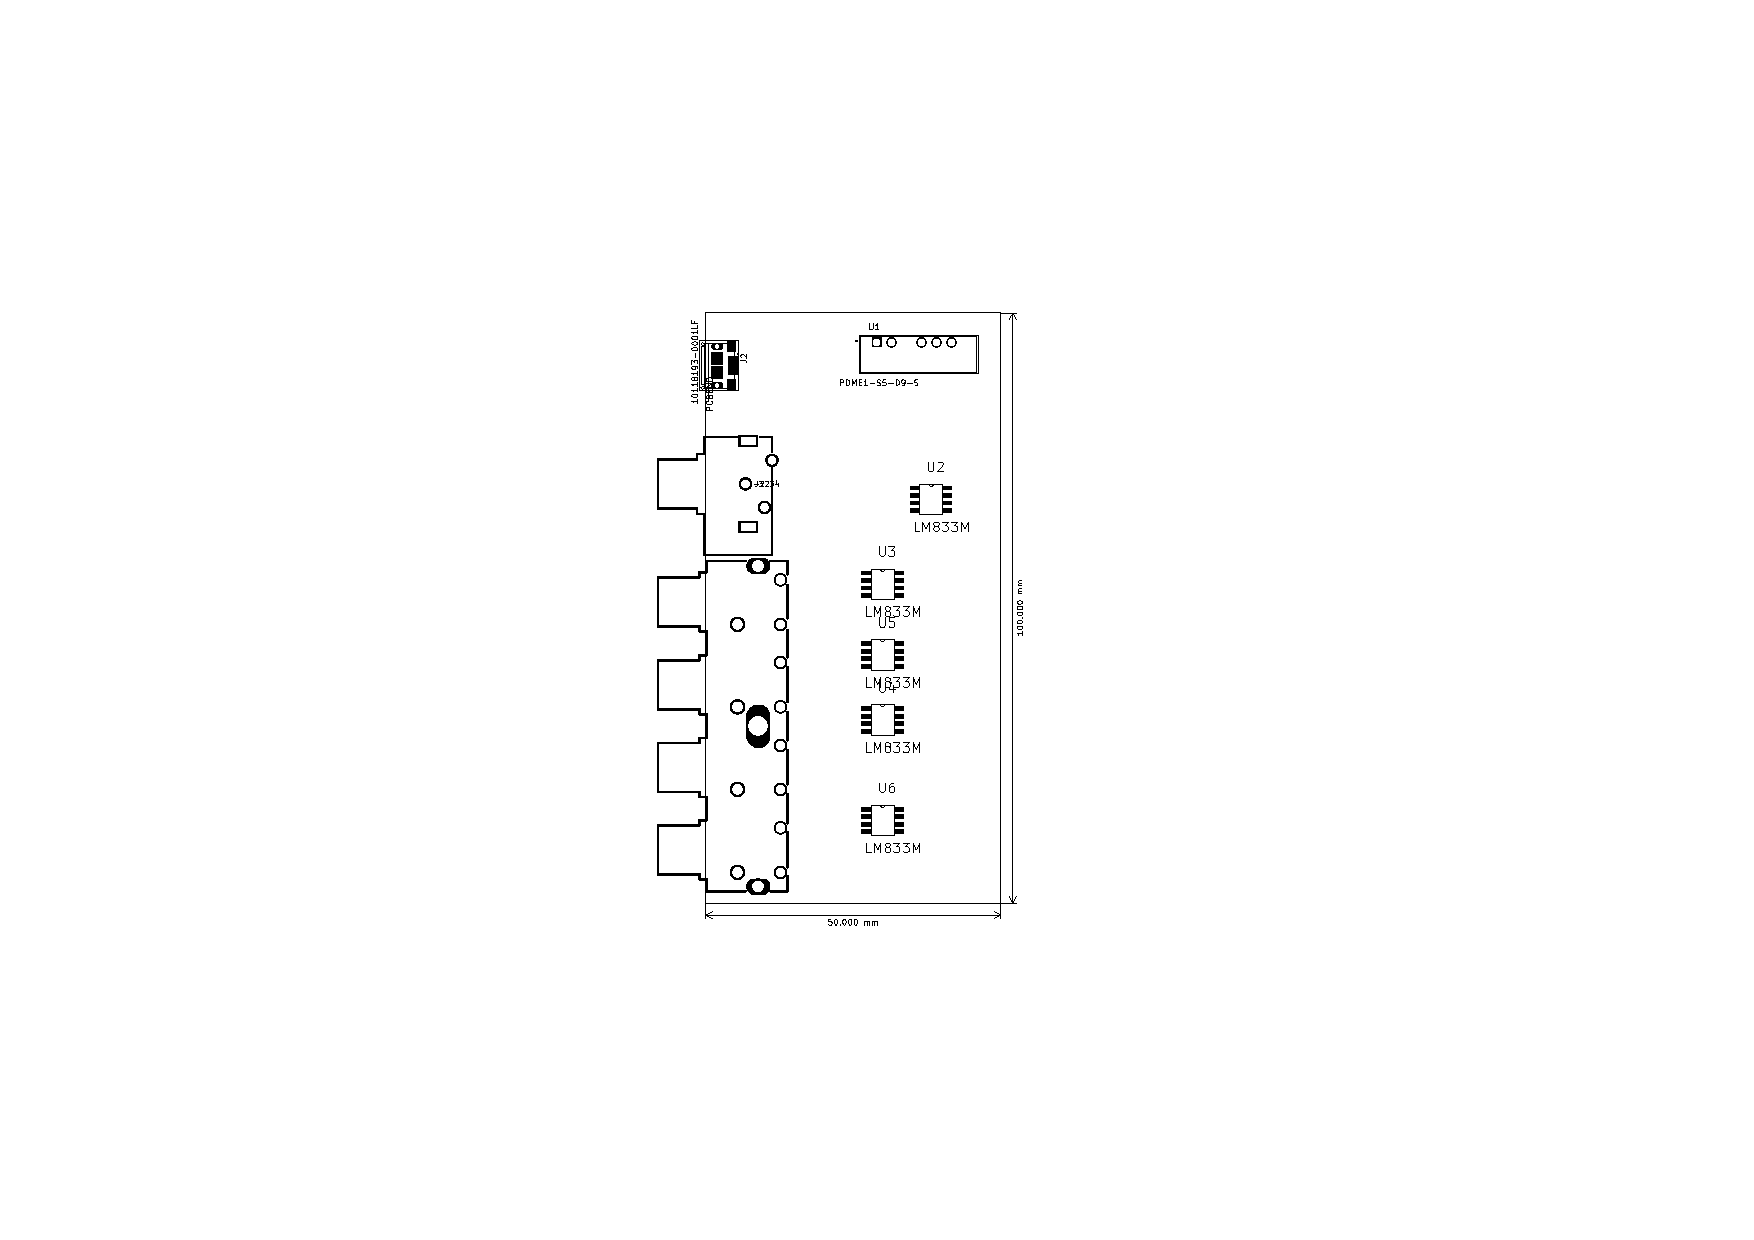
\includegraphics[trim={11cm 5cm 12cm 5cm},clip,width=6cm]{images/pcb.pdf}
\end{center}

As discussed in the design section, I have two outputs. However, I was unable to make two RCA outputs fit on the board, there simply isn't enough space. I even tried using the 3D model of the connector to see how much I can squeeze them together. To do this, I downloaded the STL file of the 3D model from the manufacturer website, and wrote a little OpenSCAD script to place them next to each other, and I tried different offsets until I found the one that would fit without any clashes. But even in squeezing them together, there simply wasn't enough space.

\begin{center}
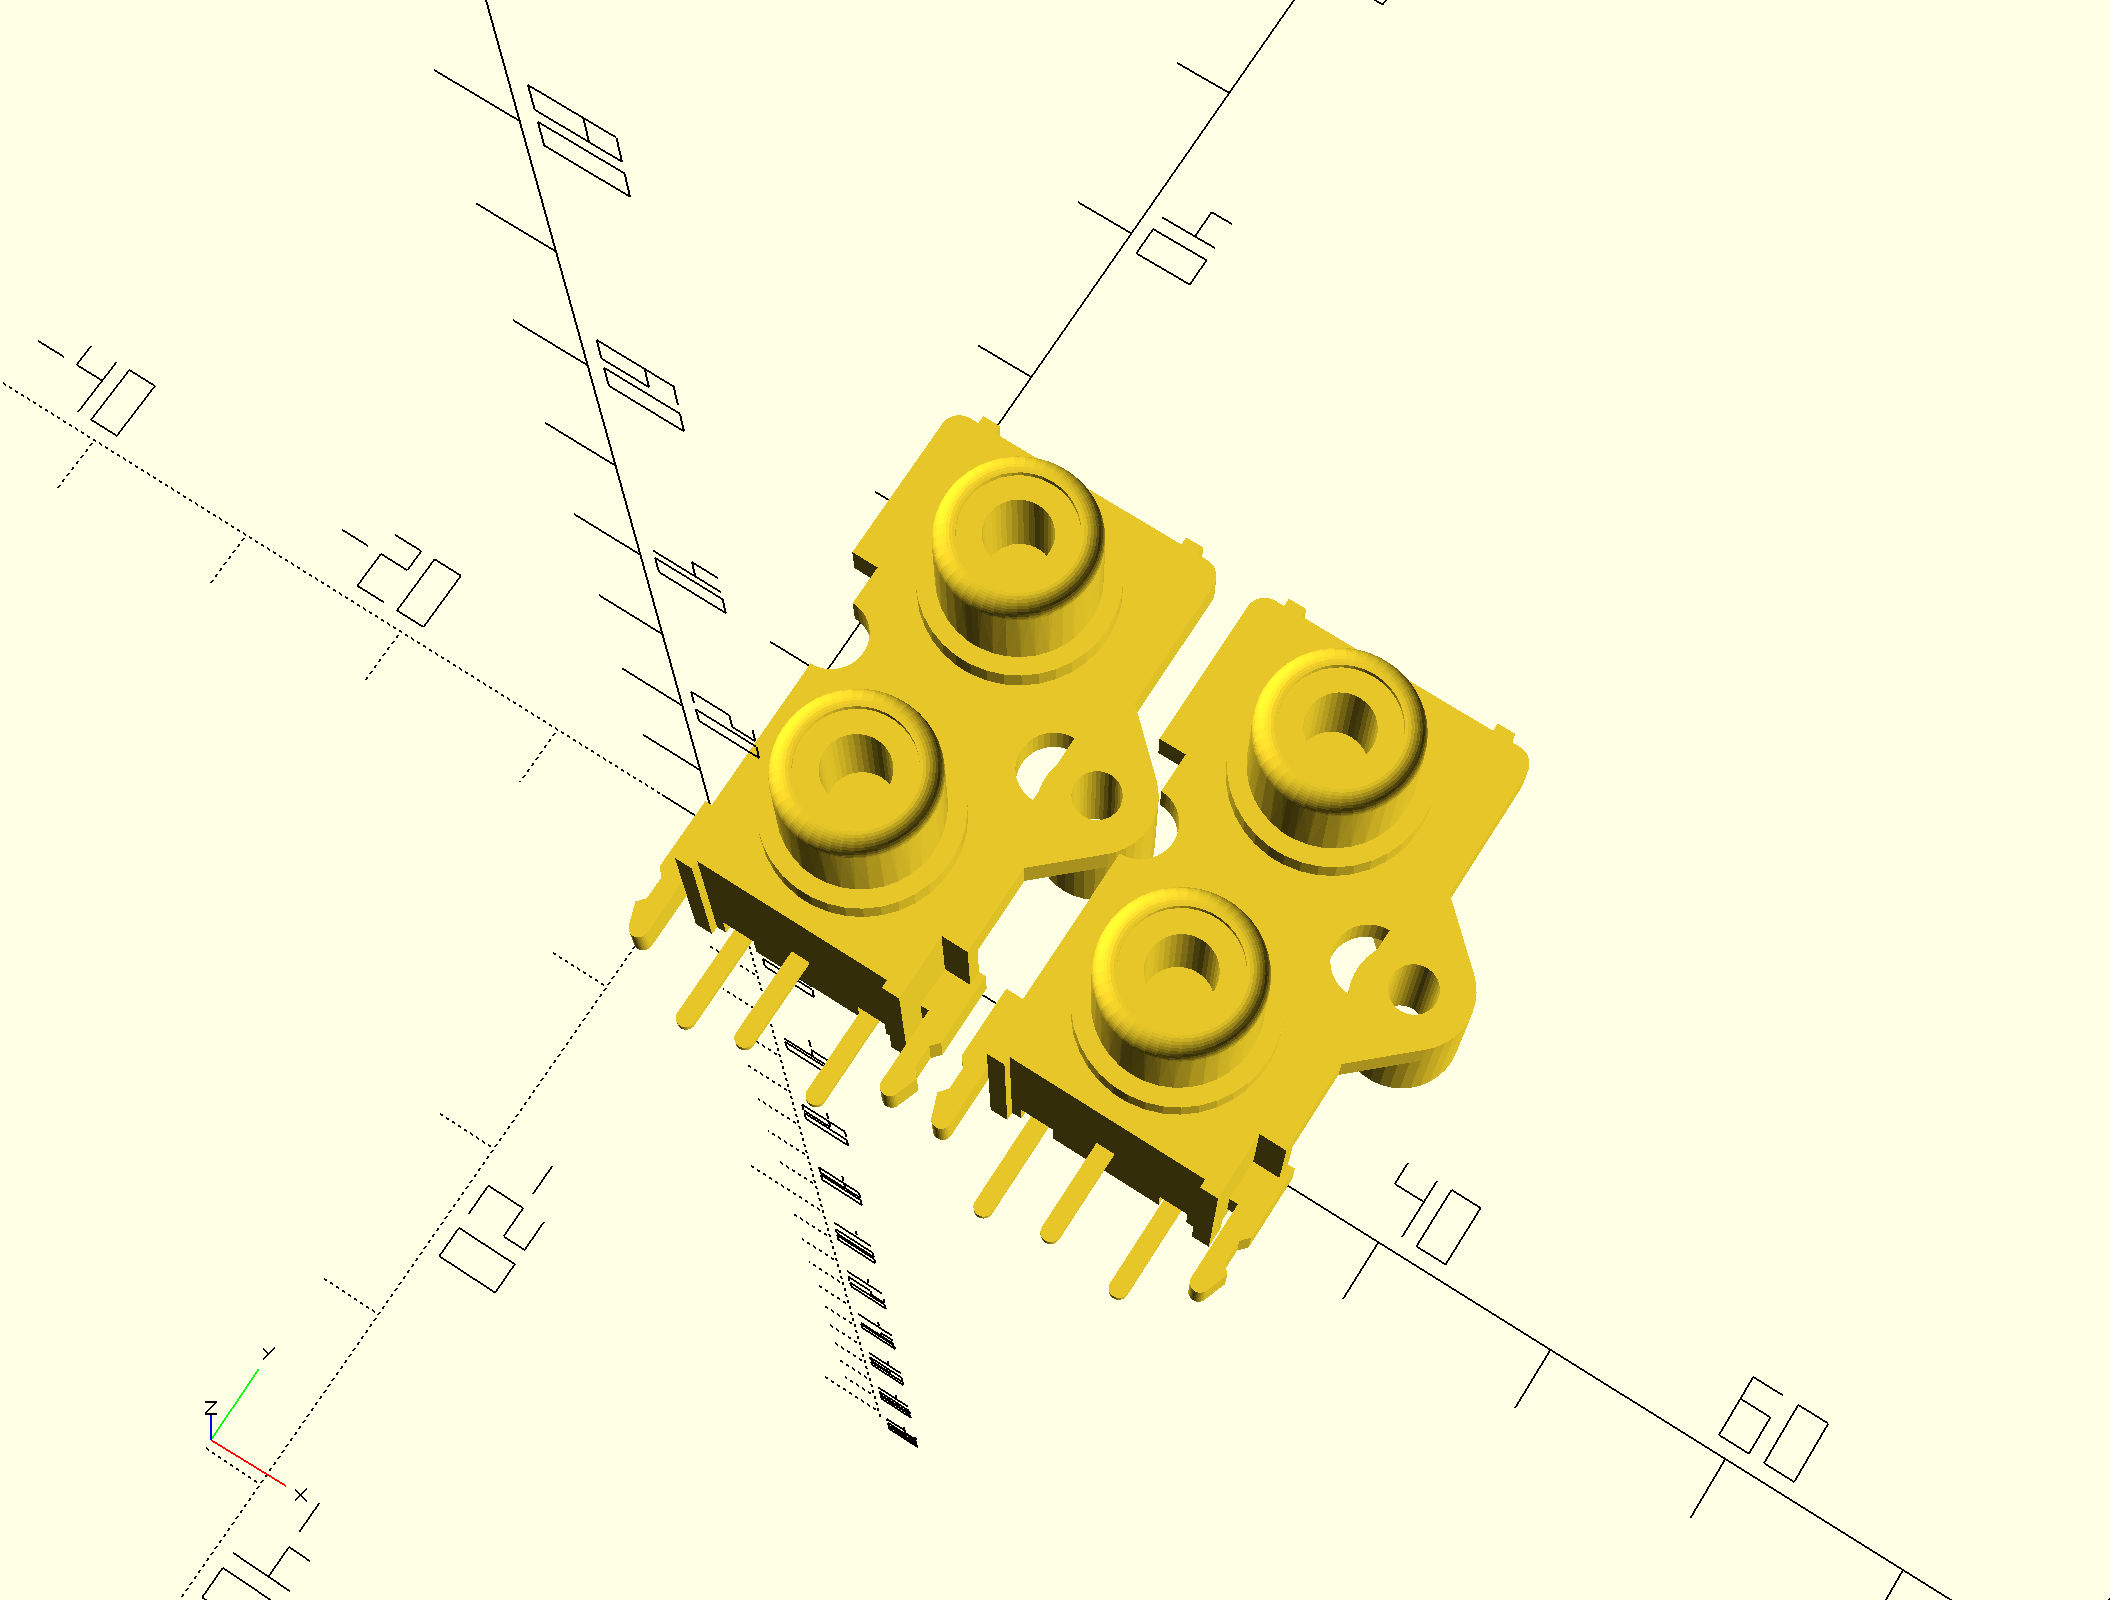
\includegraphics[width=6cm,trim={7cm 6cm 7cm 7cm},clip]{models/model}  
\end{center}

To fix this, I made a design change to change one of the output RCA jacks into a 3.5mm headphone jack.

I also had to make a custom footprint for the potentiometer, and in the process discovered that KiCad is a bit lacking when it comes to cutouts: it is not possible to create them in the GUI. I worked around that by using pins where the cutouts should be, which should also work.

I am also not entirely sure yet about the pins of the potentiometer -- since it is logarithmic, I have to use some specific pins. I have made an educated guess, but I will only know for sure when the parts arrive so that I can do some real-world testing of my circuit.

In the meantime, I was able to produce a nice looking rendering of what the board looks like thus far.

\begin{center}
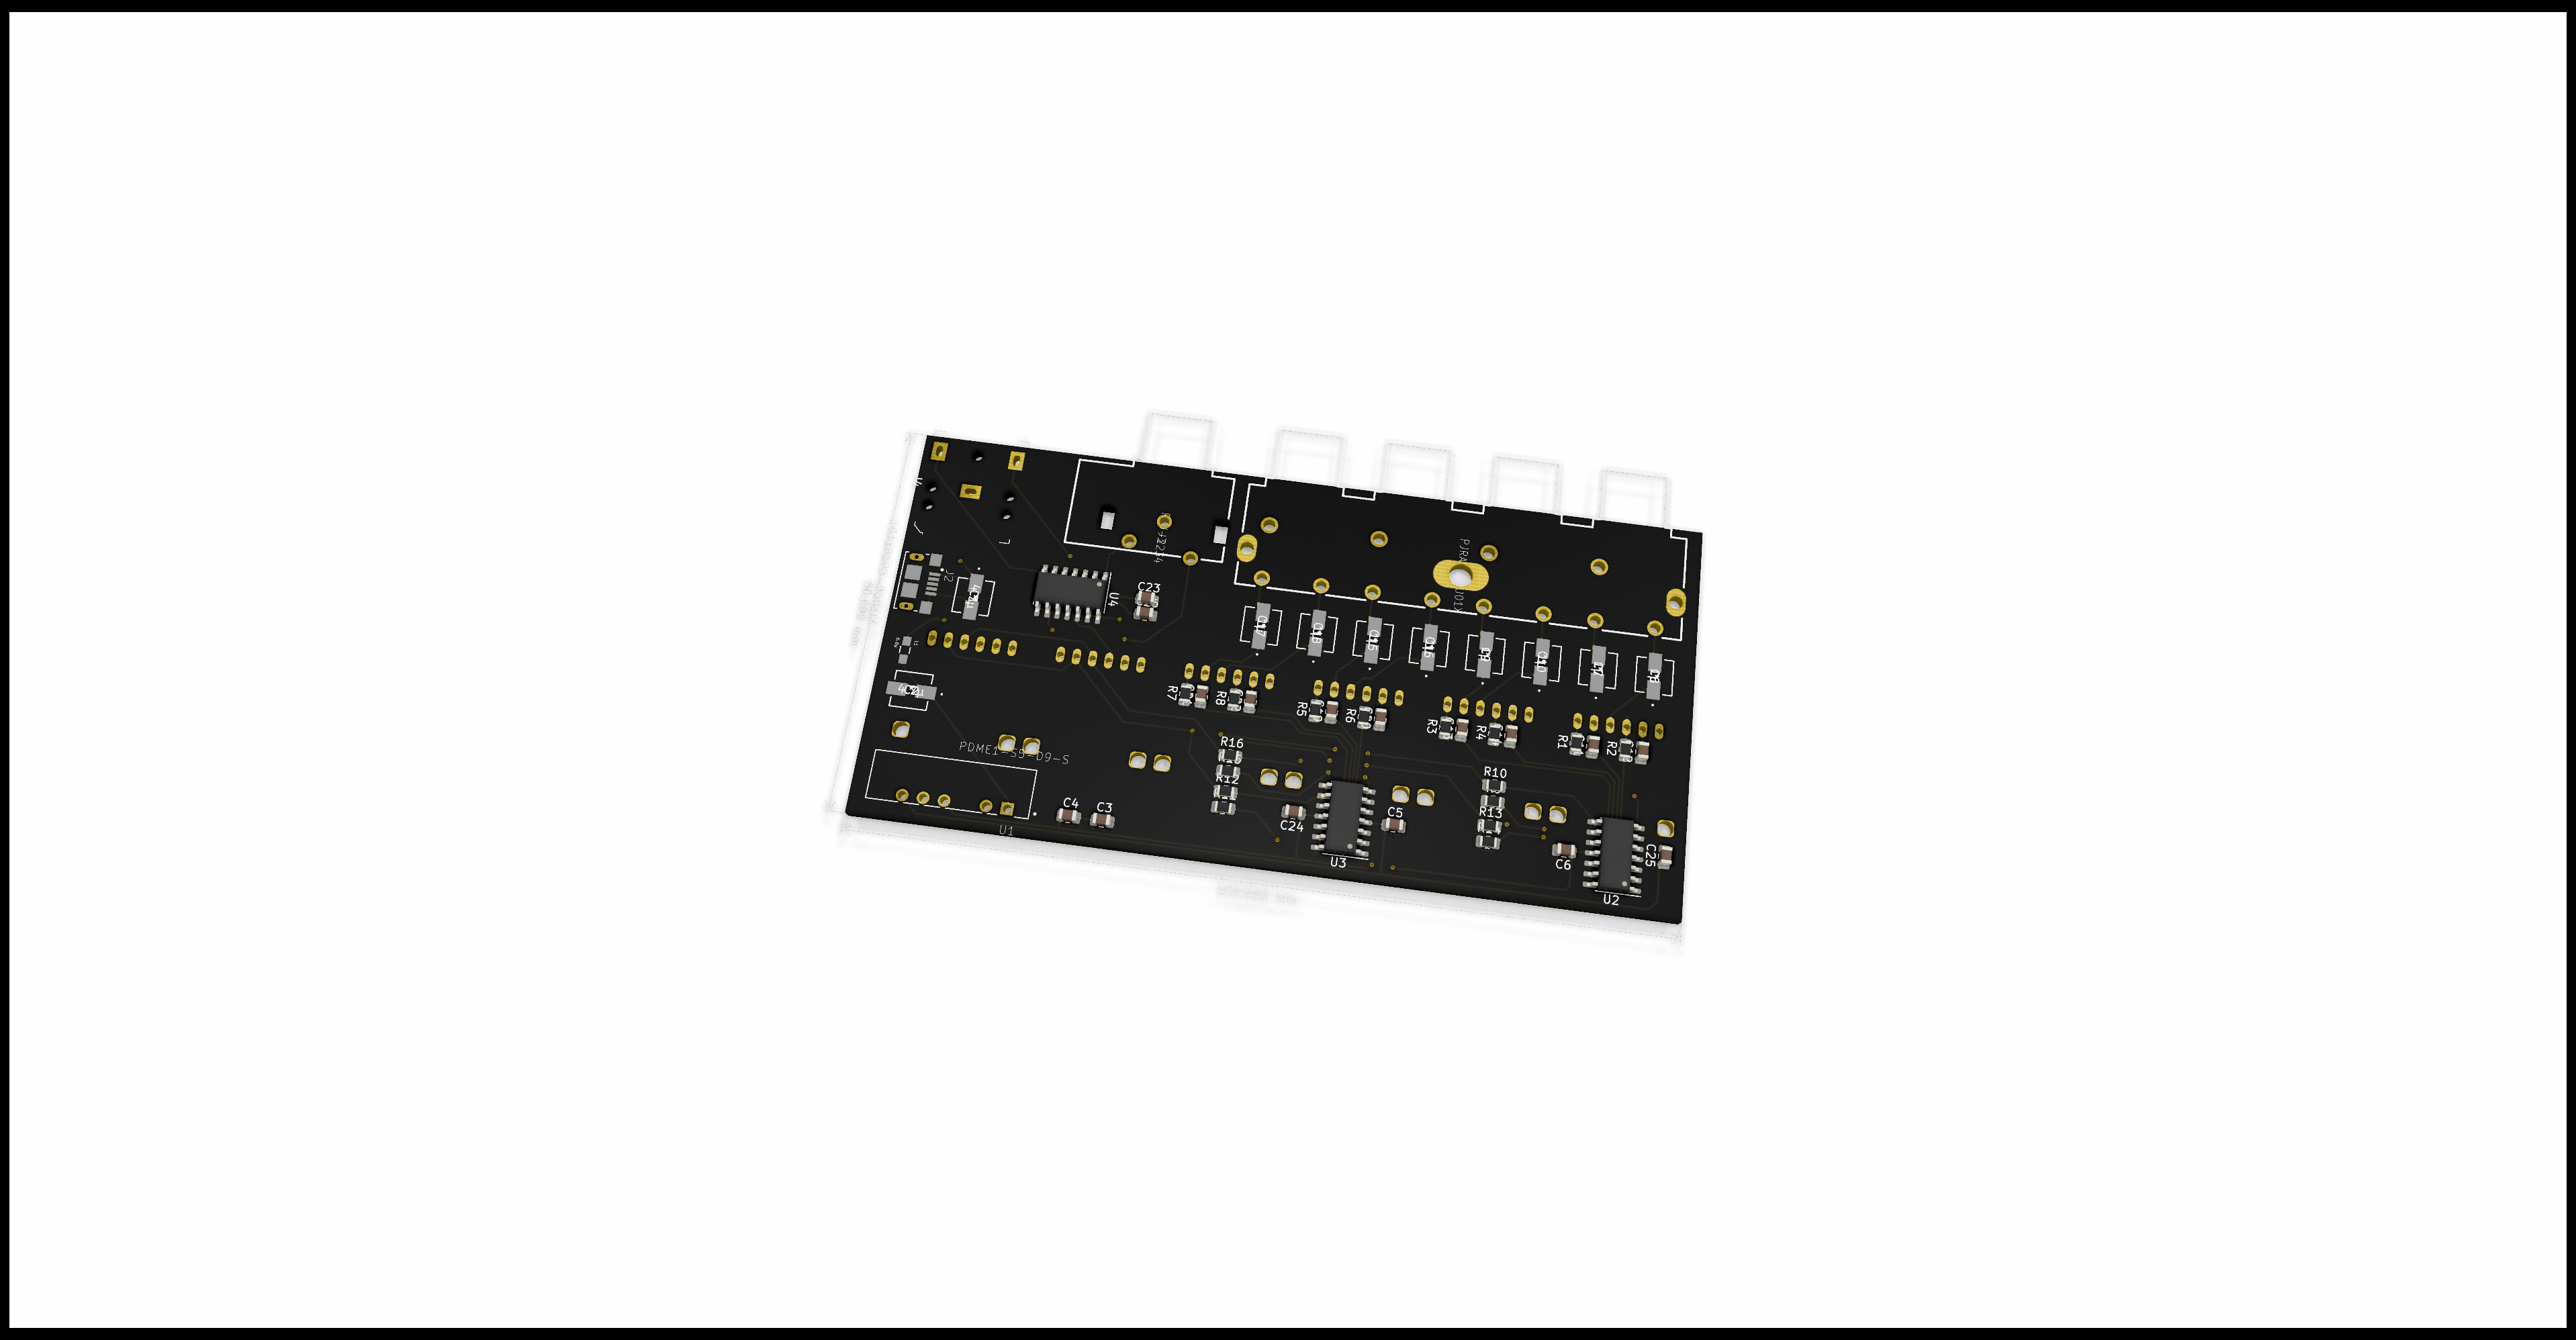
\includegraphics[width=8cm,trim={43cm 21cm 45cm 22cm},clip]{images/rendering-2019-11-09}
\end{center}

The design I chose has a number of quirks. In order to maximise efficiency, I have stuff on both sides of the PCB. One side has almost all the parts, including the RCA connectors, ICs, and so on. The other side has all of the potentiometers. 

To keep the design simple, I try to do as much on the first layer as possible, and use the second layer only as a ground plane and layer for vias where paths cross. I'm not very experienced in PCB layout and routing, and I am struggling with KiCad a bit to get things to work the way I want them to, but it should be okay. Despite being a little bit crammed, this circuit is actually very simple to layout and route.

I finished the layout and routing very quickly. I noticed a couple of issues. For once, I had put the pins for the audio jack in the wrong order.

\begin{center}
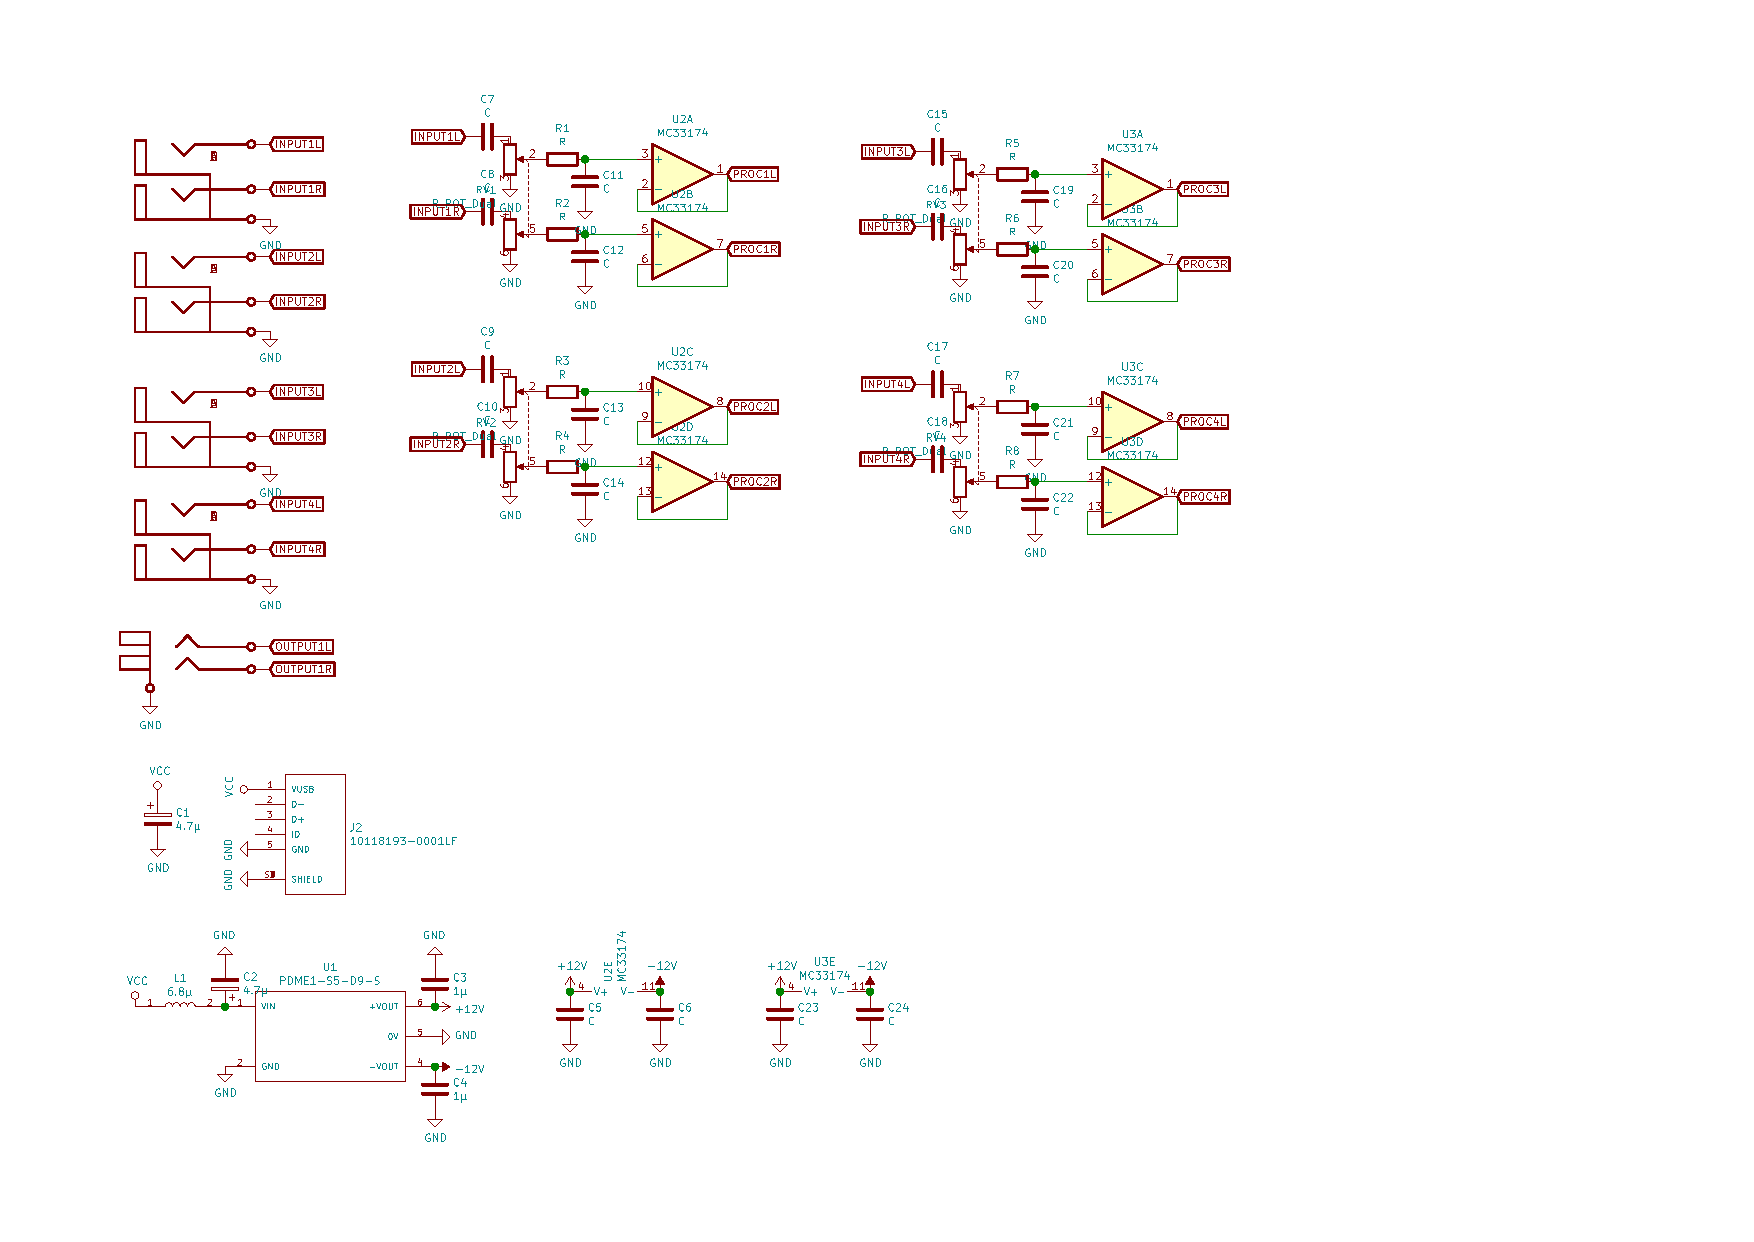
\includegraphics[width=4cm,trim={22cm 17cm 4cm 1.8cm},clip]{images/audio-mixer.pdf}
\end{center}

I verified with the datasheet to make sure that everything else is right. The datasheet clearly shows that pin 2 is the tip of the \SI{3.5}{\milli\meter} headphone jack. 

\begin{center}
\includegraphics[page=2,width=4cm,trim={2cm 7.2cm 11cm 14cm},clip]{datasheets/sj1-352xn.pdf}
\includegraphics[page=2,width=4cm,trim={5.2cm 4.2cm 13cm 21cm},clip]{datasheets/sj1-352xn.pdf}
\end{center}

I then verified in the design if this matches. In this process I also saw that I had accidentally placed the connector the wrong way, and I noticed that the holes for the plastic pins seem to be missing. From Wikipedia, I know that the tip of the connector is supposed to be the left channel, the middle bit the right channel, and the larger base ground. Based on this information, I verified the PCB layout. This is how I fixed the layout

\begin{center}
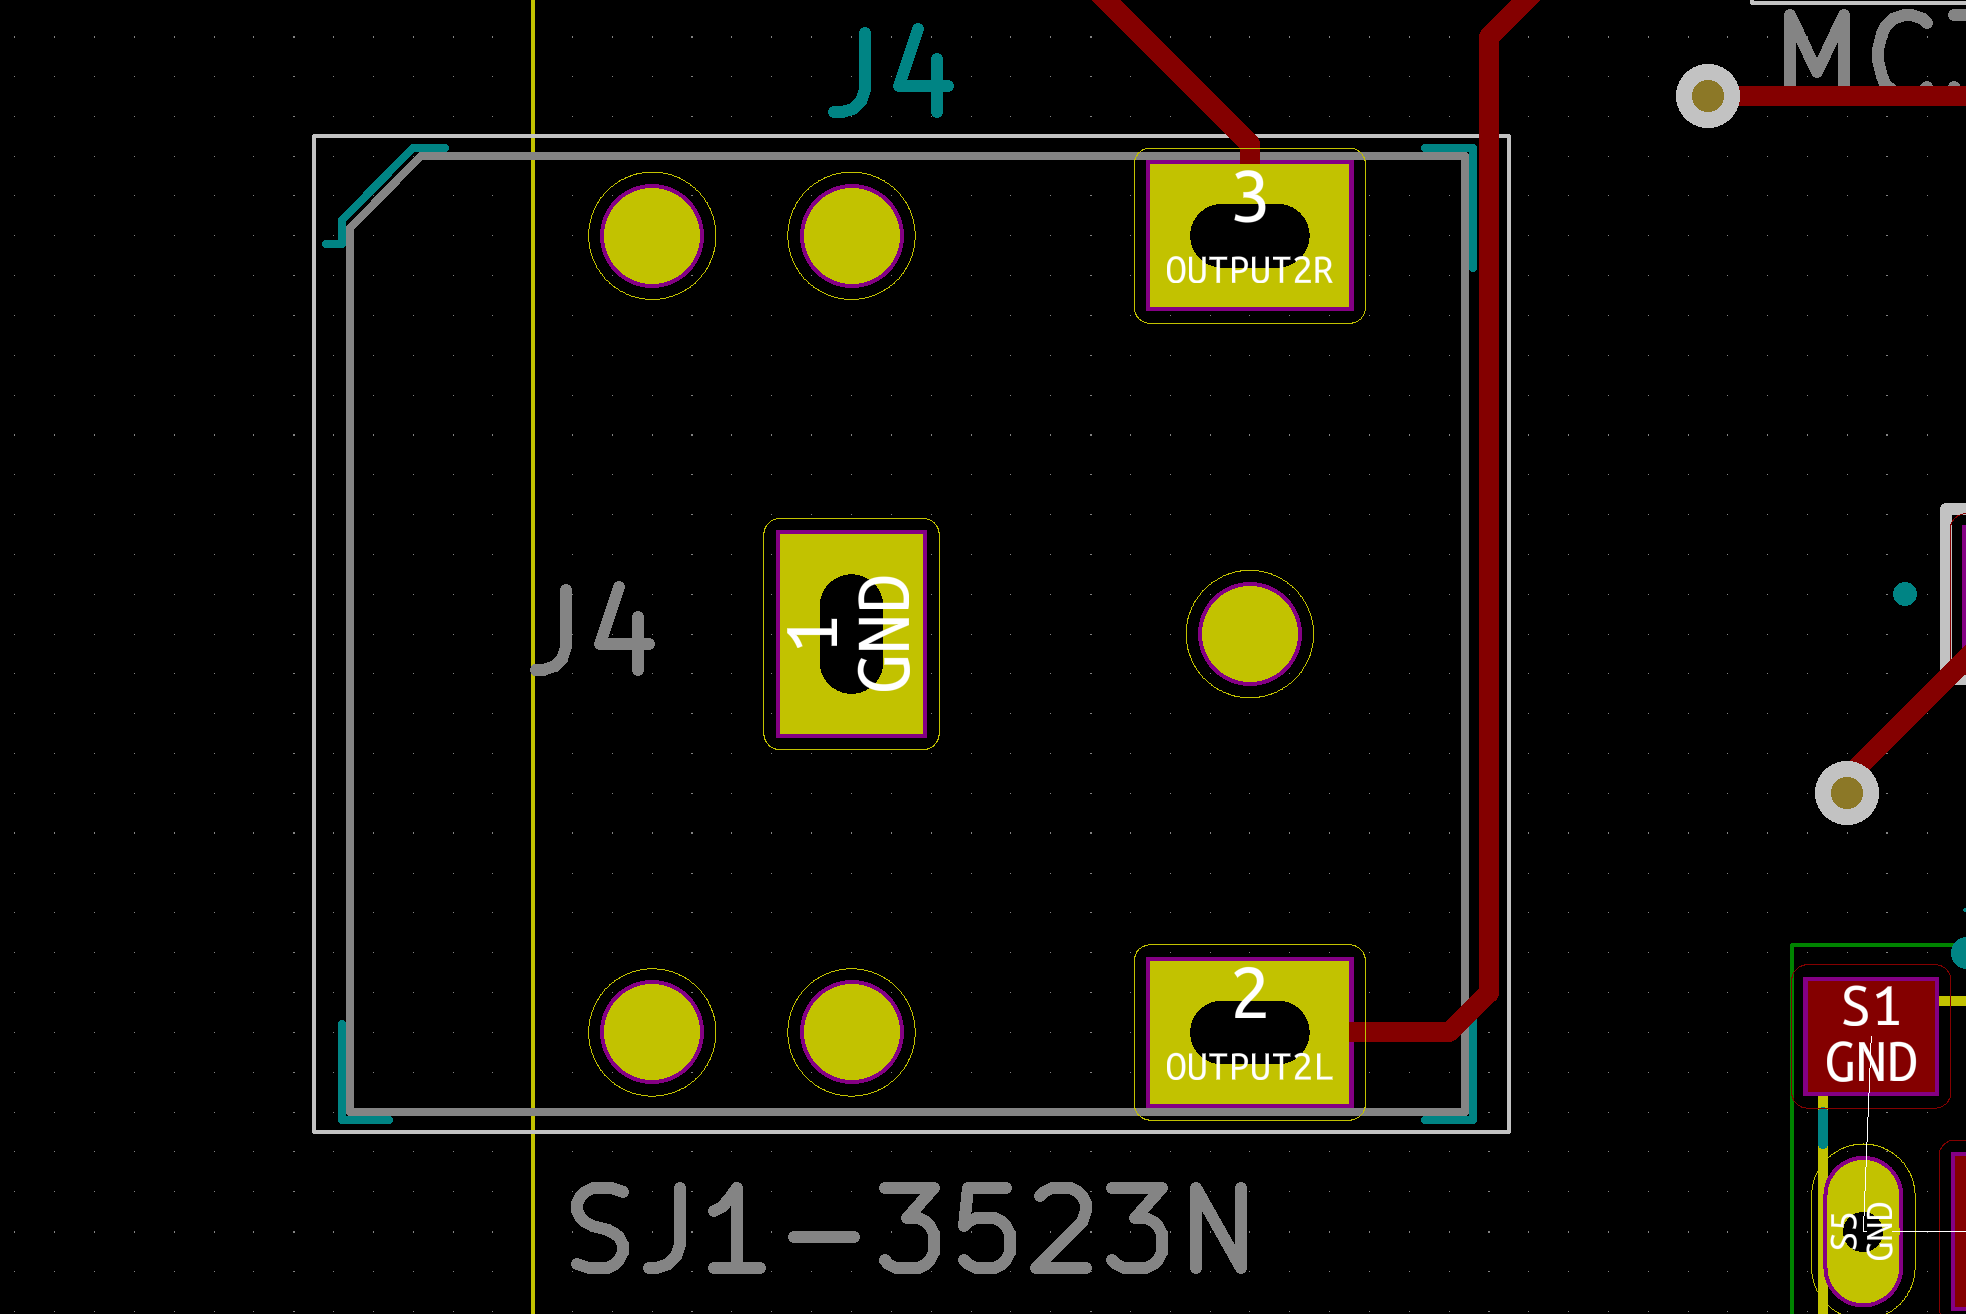
\includegraphics[width=6cm]{images/pdf-usb-connector-snap}
\end{center}

Similarly, I went through every component on the board, verifying that it is placed correctly, and that the pins are correct. This is when I noticed another issue with the board: the position of the output potentiometers does not line up with the position of the output ports. This is a small oversight I made when laying them out, I made sure to line up the input potentiometers correctly, but apparently did not take as great care with the output side. 

\begin{center}
\small
\begin{tikzpicture}
\node (pcb) {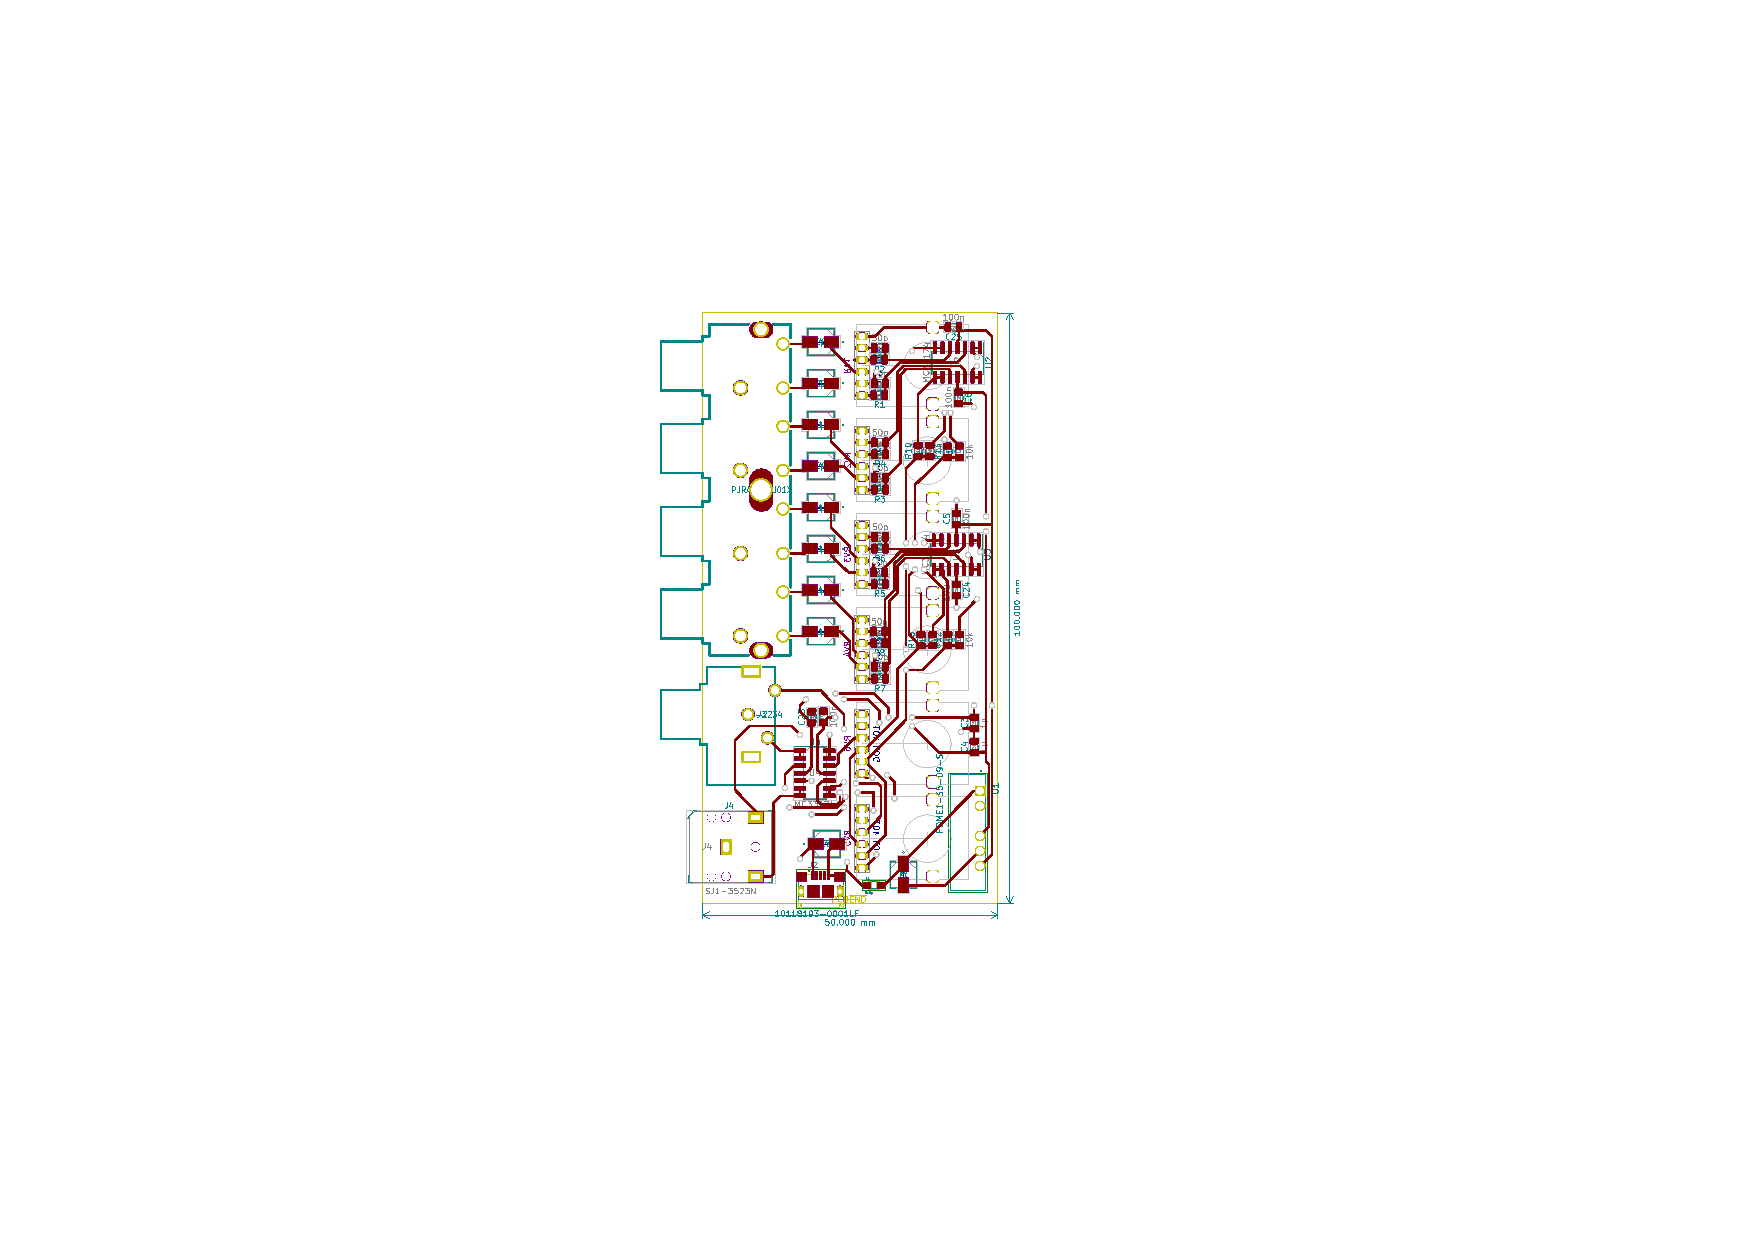
\includegraphics[width=6cm,trim={11cm 5cm 12cm 11cm},clip]{images/pcb-rev1.pdf}};
\draw (1.2,0.85) circle (2pt) ++(2pt,0) -- ++(2,0) node[anchor=west,text width=2.2cm,align=left] {Potentiometer Output 2};
\draw (1.2,-0.6) circle (2pt) ++(2pt,0) -- ++(2,0) node[anchor=west,text width=2.2cm,align=left] {Potentiometer Output 1};
\draw (-1.8,1.3) circle (2pt) ++(-2pt,0) -- ++(-1.5,0) node[anchor=east] {Output 1};
\draw (-1.8,-0.7) circle (2pt) ++(-2pt,0) -- ++(-1.5,0) node[anchor=east] {Output 2};
\end{tikzpicture}
\end{center}

This is something I need to fix in the next revision. The physical inputs, outputs and knobs should ideally line up. In the next revision, I might also change the position of the USB power input.

\subsection{First Prototype Manufacture}

As I was expecting, there were some issues in the first prototype already. Thankfully, the issues were minor enough that I was able to actually assemble a prototype that was more or less working, to verify that the circuit generally works. Most of the issues had to do with part footprints being incorrect.

% https://sound-au.com/articles/capacitors.htm

For the \SI{3.5}{\milli\meter} audio jack, there were holes drilled for little plastic spacers, however these are intended to be spacers from the PCB and do not require holes to be drilled.

% FIXME: insert picture of drilled holes

I fixed this by opening up the part, and changing it to remove the holes. Instead, I put little circles on the user information layer to indicate the position of them.

\begin{center}
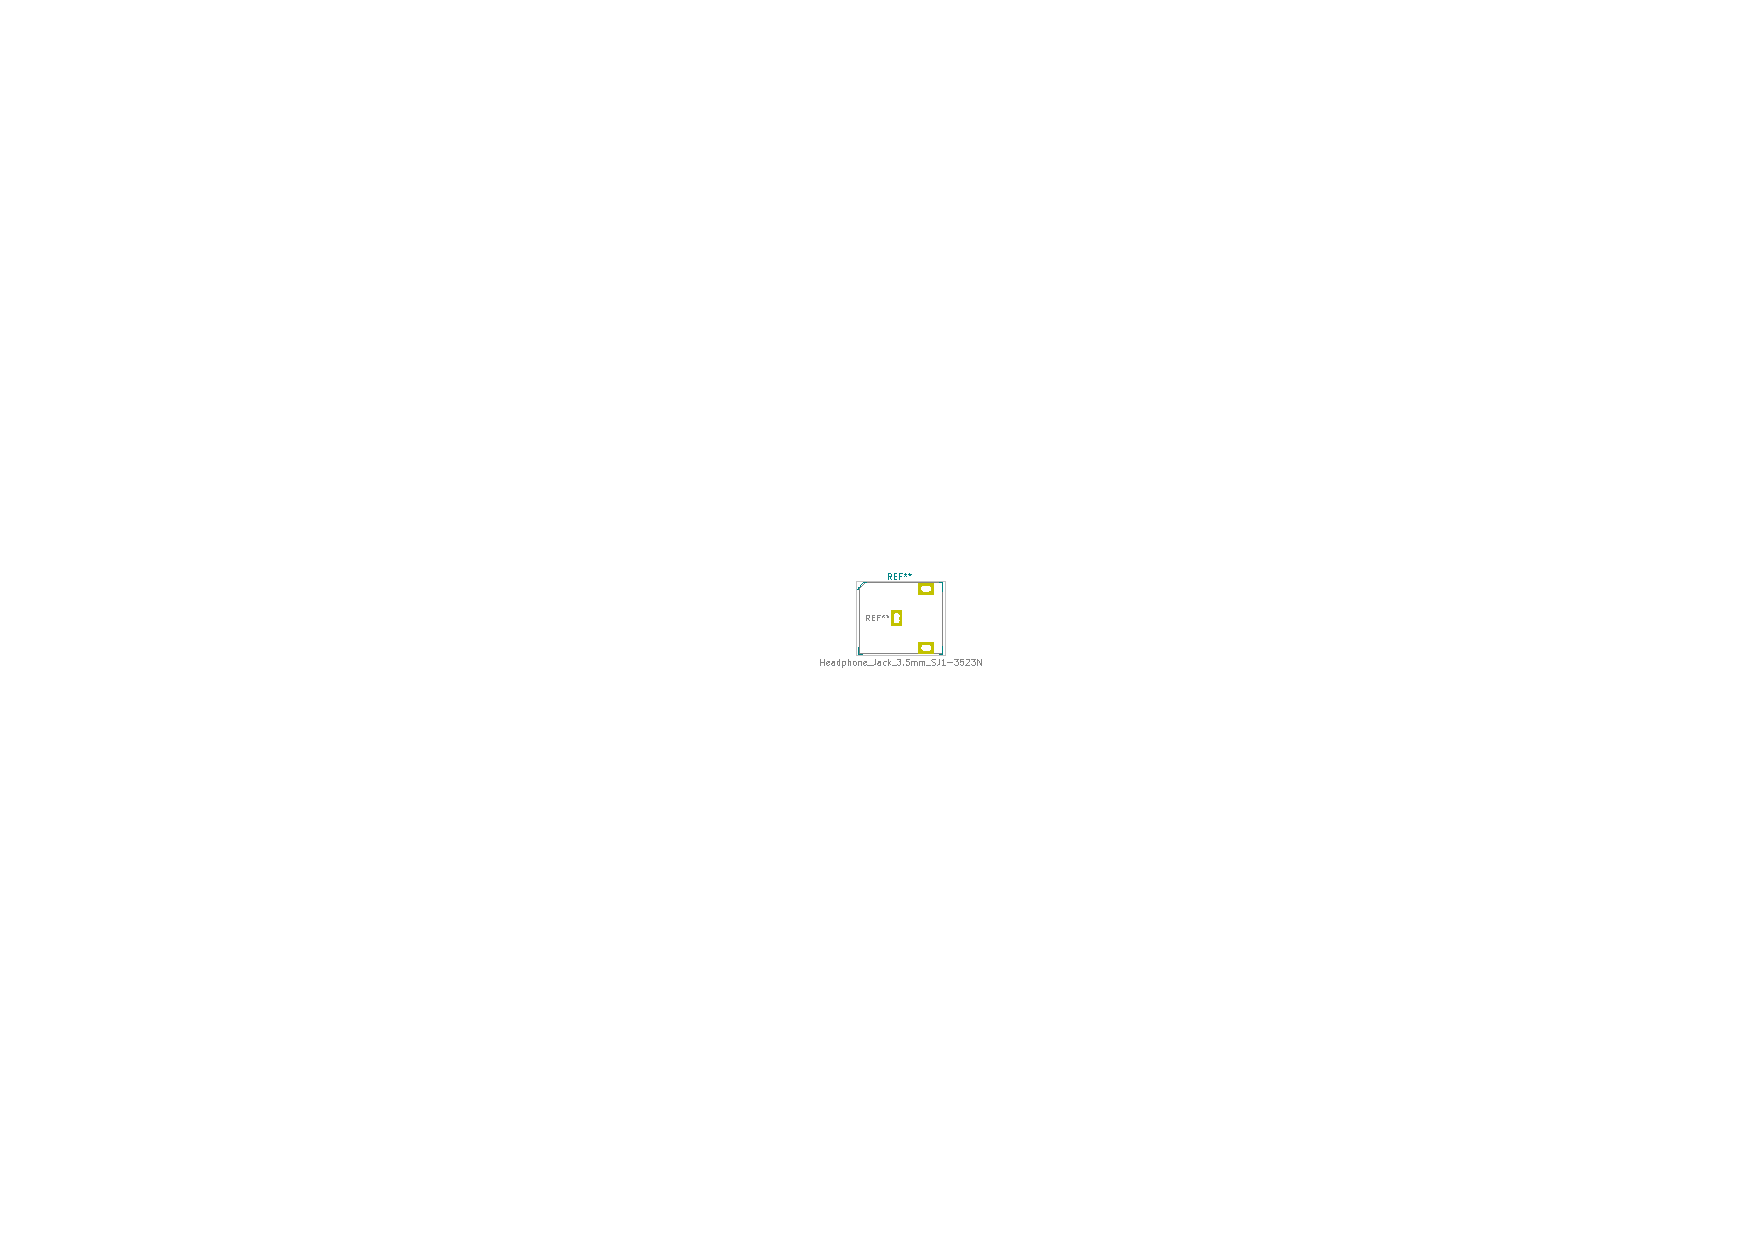
\includegraphics[height=3cm,trim={13.7cm 9.7cm 13cm 9.7cm},clip]{images/headphone-jack-bad.pdf}
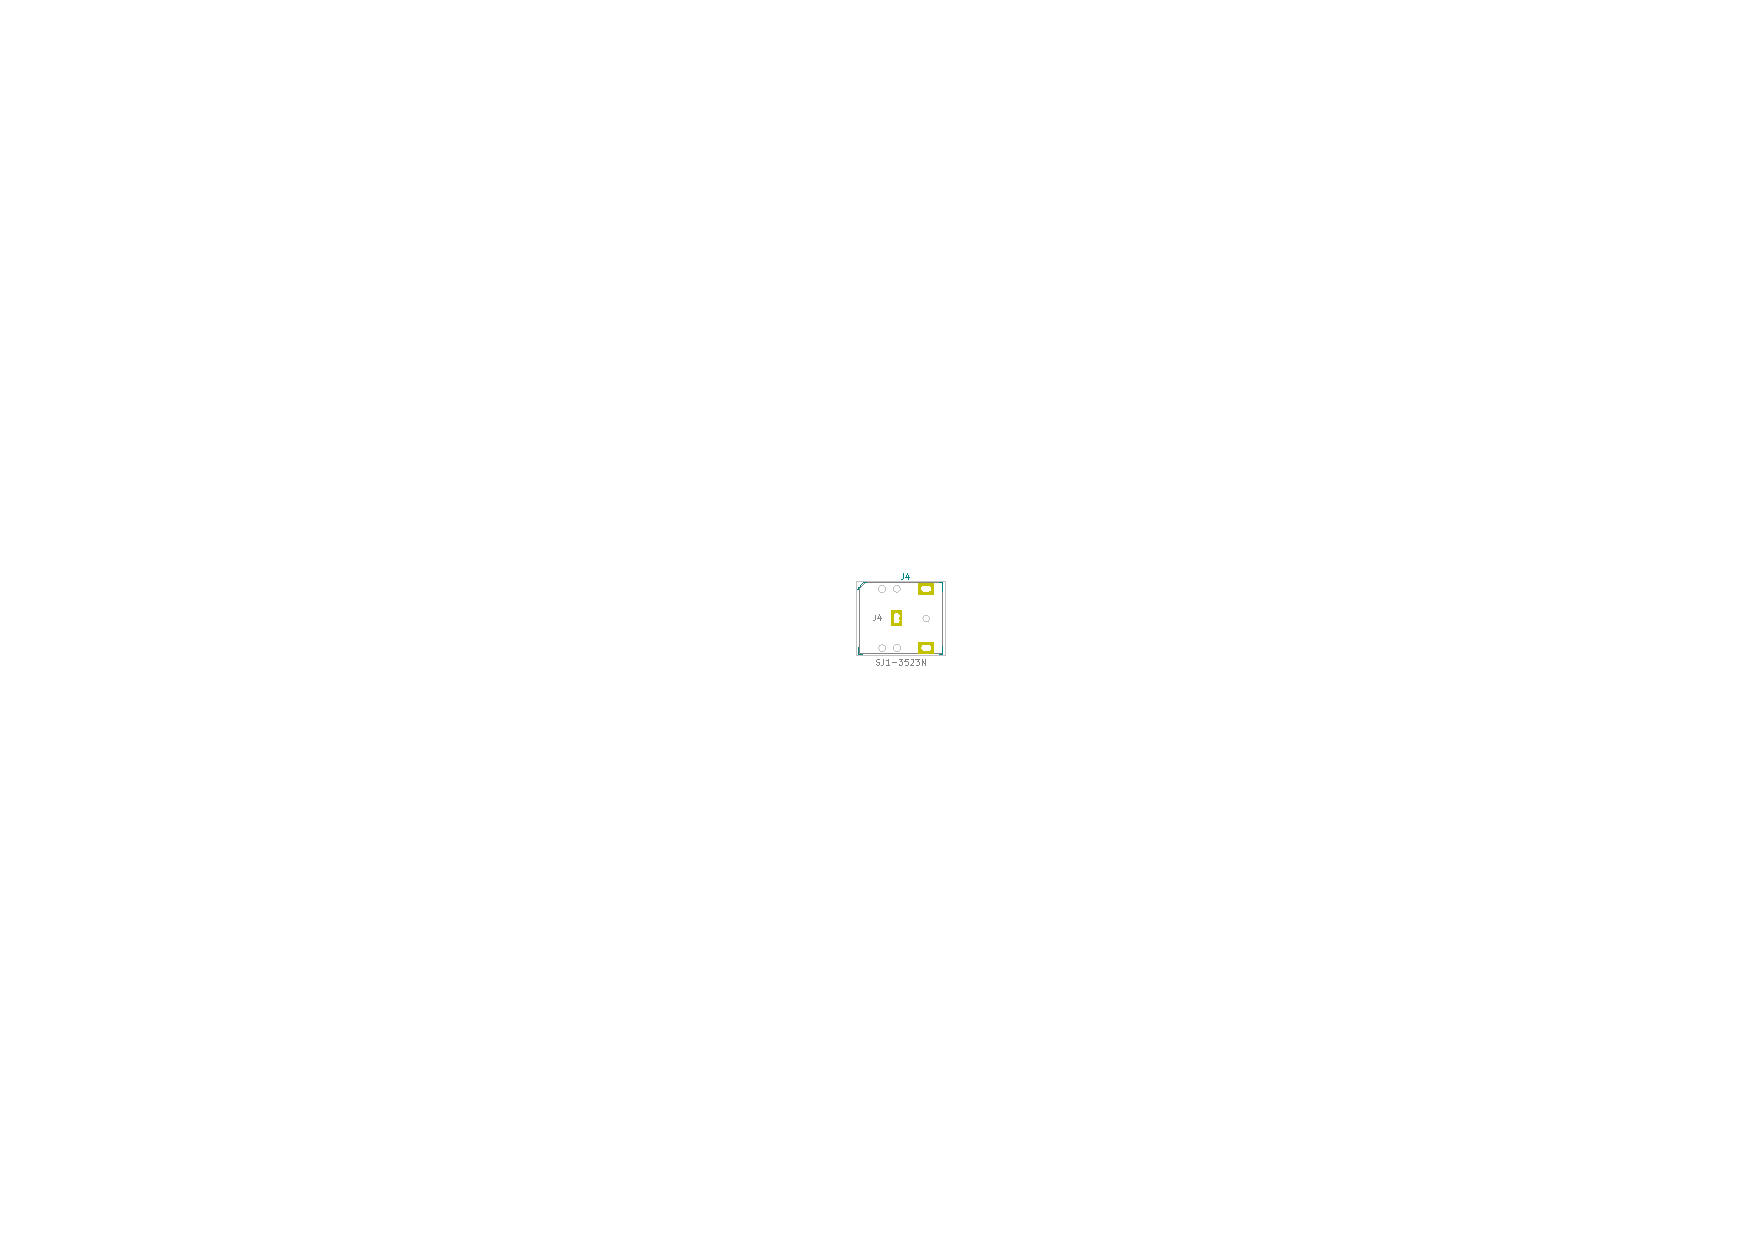
\includegraphics[height=3cm,trim={14.5cm 9.7cm 13.7cm 9.7cm},clip]{images/headphone-jack-fixed.pdf}
\end{center}

While at it, I decided to also add more holes in order to accomodate other headphone jacks -- there is another style that has five pins instead of three, where the other two pins act as a switch that is activated upon insertion of the plug. I don't need this feature, but it is useful to be able to support both styles.

% TODO: add pad, add picture

The large four-channel stereo input RCA jack connector had bad incorrect holes cutout for the plastic tabs. The holes were far too small, which I was able to mitigate by cutting off the plastic tabs to get a working prototype.

% TODO: fix footprint, add picture.

The potentiometers have a detent in the center of their output. This is not really desireable, unless I use that for something (such as making that the unamplified level).

I think that the logarithmic taper is inverted for the two channels, such that this pot can be used for balancing. That is definitely \emph{not} what I want. Thus, I looked for alternatives, and found a pot that might do what I want, and has the additional advantage of being cheaper.

% TODO: show alternative pot

% switch to using cheaper https://www.mouser.de/ProductDetail/ALPS/RK12L12C0A0G?qs=sGAEpiMZZMtC25l1F4XBU%2FgM1eD5hBFTeDAcQkh0Ztk%3D

The potentiometers had holes for the metal tabs that were just slightly too small. They had to be bent slightly to be made to work and fit. 

I fixed this by increasing the drill size, such that they would fit better.

The two \SI{5}{\volt} input rail capacitors had incorrect markings on the PCB (polarity reversed). The marking on the caps denotes the negative polarity. This error was made because I did not use polar caps in the schematic where I should have, and the footprints were wrong (at least I think they were). To remedy this, I switched to another style of footprint that is in the KiCad default library.

I was unable to correctly put together the end stages because I did not have \SI{50}{\kilo\ohm} resistors at hand. I was able to mitigate by using \SI{100}{\kilo\ohm} resistors instead, slightly increasing the attenuation. 

The most severe issue, however, was that the pins of the potentiometer were assigned wrong. One of the channels is flipped, such that the left channel is at max when turning them all the way down, and the right channel is at max when turning them all the way up. I had apparently made an error when measuring the channels.

% https://forum.kicad.info/t/create-a-mounting-hole/6737

Another thing I noticed is that it would make sense to add holes on the corners of the PCB, this makes mounting easier. It seems like an M3 size mounting hole is ideal. I did this by using the M3 mounting hole provided in the KiCad library. I had some issues squeezing them on the PCB, but managed to do so by moving some components around slightly.

\section{Fabrication}

% https://jlcpcb.com/client/index.html#/parts

\section{Orders}

\subsection{2019-11-09}

Today I ordered components for the prototype boards. The boards are not yet designed, but I wanted to get the components ahead of time, so that I could do a bit of testing before sending the PCBs out for manufacture.

It ended up being a bit more expensive that I anticipated, at around 90\,€. I ordered many parts in very large quentities, like the SMD resistors, because they are cheap and can be used for other projects as well. The other components were chosen such that I have at least enough for two fully assembled boards. Table \ref{tbl:order-2019-11-09} shows the bill of this first order from Digikey.

\begin{table}[p]
\thisfloatpagestyle{empty}
\centering
\vspace*{-2cm}
\caption{First order from Digikey}\label{tbl:order-2019-11-09}
\newcommand{\partline}[7]{
#1&Part&#2&#3&#4&#5\\
&Manufacturer Part&#6\\
&Description&#7\\}
\footnotesize
\begin{tabular}{@{}llp{5cm}lrr@{}}
\toprule
&&&Amount&Price&Total\\
\midrule
\partline{1}{311-10.0KCRCT-ND}{100}{0.0131}{1.31}{RC0805FR-0710KL}{RES SMD 10K OHM 1\% 1/8W 0805}
\midrule
\partline{2}{311-100KCRCT-ND}{100}{0.01380}{1.38}{RC0805FR-07100KL}{RES SMD 100K OHM 1\% 1/8W 0805}
\midrule
\partline{3}{MC33274ADR2GOSCT-ND}{10}{0.69700}{6.97}{MC33274ADR2G}{IC OPAMP GP 4 CIRCUIT 14SOIC}
\midrule
\partline{4}{1276-1007-1-ND}{100}{0.01590}{1.59}{CL21F104ZBCNNNC}{CAP CER 0.1UF 50V Y5V 0805}
\midrule
\partline{5}{493-9794-1-ND}{24}{0.17900}{4.30}{UWJ1E4R7MCL1GB}{CAP ALUM 4.7UF 20\% 25V SMD}
\midrule
\partline{6}{102-6322-ND}{5}{0.15800}{10.79}{PDME1-S5-D12-S}{DC-DC ISOLATED 1 W 4.5-5.5 VDC}
\midrule
\partline{7}{1276-6470-1-ND}{20}{0.08000}{1.60}{CL21B105KBFNNNG}{CAP CER 1UF 50V X7R 0805}
\midrule
\partline{8}{445-6402-1-ND}{10}{0.11500}{1.15}{MLZ2012M6R8WT000}{FIXED IND 6.8UH 350MA 400 MOHM}
\midrule
\partline{9}{P2J4103-ND}{12}{0.19600}{14.35}{EVJ-YK6F03651}{POT 10K OHM 1/20W LOGARITHMIC}
\midrule
\partline{10}{609-4616-1-ND}{5}{0.38000}{1.90}{10118193-0001LF}{CONN RCPT USB2.0 MICRO B SMD R/A}
\midrule
\partline{11}{SC1537-ND}{2}{0.79000}{7.58}{PJRAS4X2U01X}{CONN RCA JACK MONO 3.2MM R/A}
\midrule
\partline{12}{102-5864-ND}{5}{0.23000}{6.15}{RCJ-2233}{CONN RCA JACK DUAL R/A WHT/WHT}
\midrule
\partline{13}{CP1-3523N-ND}{4}{0.66000}{2.64}{SJ1-3523N}{CONN JACK STEREO 3.5MM R/A}
\midrule
\partline{14}{PCE4301CT-ND}{24}{0.22900}{5.50}{EEE-1HA010NR}{CAP ALUM 1UF 20\% 50V SMD}
\midrule
\partline{15}{1276-1156-1-ND}{100}{0.02140}{2.14}{CL21C470JBANNNC}{CAP CER 47PF 50V C0G/NP0 0805}
\midrule
&&&&Sum&69.35\\
&&&&Taxes&13.18\\
&&&&Total&82.53\\
\bottomrule
\end{tabular}
\end{table}

I've set my limit for the budget of this project to something like 500\,€, which should be sufficient to get me going at least. I might not even need that much. If I come up with anything useful at all, I could sell it to people as kits and get some of my money back, but that depends on a lot of factors, so I don't really expect it to work out. Also, this project is probably rather expensive for people, as this is my first time designing anything, I don't yet have a whole lot of experience in reducing the BOM cost.

\subsection{2019-11-13}

\begin{table}[h!]
\centering
\caption{First order from JLC PCB}\label{tbl:order-2019-11-09}
\newcommand{\partline}[7]{
#1&Part&#2&#3&#4&#5\\
&Manufacturer Part&#6\\
&Description&#7\\}
\footnotesize
\begin{tabular}{@{}llp{5cm}lrr@{}}
\toprule
&&&Amount&Price&Total\\
\midrule
1 & Part & PCB Samples & 10 & 4.54 & 4.54\\
& Layers & 2\\
& Size & \SI{100}{\milli\meter} by \SI{50}{\milli\meter}\\
& Thickness & \SI{1.6}{\milli\meter}\\
& Color & Black\\
& Surface finish & HASL (with lead)\\
\midrule
&&&&Sum&4.54\\
&&&&Shipping&17.58\\
&&&&Total&22.12\\
\bottomrule
\end{tabular}
\end{table}

Today I ordered the PCB samples of the first build. This is exciting.

\section{Conclusion}

I learned a lot of things in this project. It is very easy to design simple analog audio circuits using building blocks like opamps, and by following the datasheet recommendations for rail filtering capacitors. 

Because KiCad is open source software, it has a few rough edges where commercial software is maybe more polished. The biggest issue I found was that some of the footprints had errors in them, which I had to correct manually. 

This is not a huge deal, because I found that it was generally not that difficult to fix footprints or even make custom ones. This is better than using ones from the internet, because making them custom means that you can make sure all the measurements and hole sizes are exactly correct.

Using services like JLCPCB and Digikey, it is easy to order parts even in low quantities and have a PCB manufactured for testing. I was very surprised at the low cost of the bare PCBs.

For the components, sourcing is not always easy. It is difficult to find parts that are affordable, available in small quantities, and that do exactly what is needed. Also, sometimes parts have missing or incomplete documentation, which can lead to design errors (like for the potentiometers, which did not document the position of their tapers to my satisfaction). For these types of issues, prototypes are vital to check if things work together as expected.

\end{document}